\documentclass[lettersize,journal]{IEEEtran}
\usepackage{amsmath,amsfonts}
\usepackage{algorithmic}
\usepackage{array}
\usepackage[caption=false,font=normalsize,labelfont=sf,textfont=sf]{subfig}
\usepackage{textcomp}
\usepackage{stfloats}
\usepackage{url}
\usepackage{verbatim}
\usepackage{graphicx}

\usepackage{lipsum}
\usepackage{mathtools}
\usepackage{cuted}

\usepackage{array}
\usepackage{graphicx}
\usepackage{cite}
\usepackage{subfigure}
\usepackage{amsmath,amssymb,amsthm}
\usepackage[indent,bf]{caption2}
\usepackage{rotating}
\usepackage{setspace}
\usepackage{longtable}
\usepackage{comment}
\usepackage{float}
\usepackage{hyperref}
\usepackage{cleveref}
\usepackage{graphicx}
%\newcommand{\crefrangeconjunction}{ to~}
\usepackage{subcaption}
\usepackage{enumitem}
\usepackage{pgfgantt}
%\usepackage{longtable}
 \usepackage{dingbat}
% \usepackage{verbatim}
\usepackage{amssymb}

\setcounter{MaxMatrixCols}{20}

%-------------------------------- Defitions
\def \SE {\textbf{SE}(3)}
\def \SO {\textbf{SO}(3)}
\def \se {\textbf{se}(3)}
\def \so {\textbf{so}(3)}
\def \R  {\mathbb{R}}
\def \g  {\mathfrak{g}}
\def \q  {\mathfrak{q}}
\def \m  {\mathfrak{m}}

\def \V {\mathcal{V}}
\def  \I {\mathcal{I}}
%\def  \or {\mathcal{o}}
\def  \B {\mathcal{B}}
\def \Ad {\textbf{Ad}}
\def \Add {\mathfrak{Ad}}
\def \L {\mathcal{L}}
\def \A {\mathcal{A}}
\def \O {{}^0\Omega^I_{loc}}
\def \sin {\textbf{sin}}
\def \cos {\textbf{cos}}

\def \diag {\text{diag}}

\newtheorem{theorem}{Theorem}
\newtheorem{lemma}{Lemma}
\renewcommand{\qedsymbol}{$\blacksquare$}
% \newtheorem{example}{Example}


%\newcommand{example}{\large \subsection}
\theoremstyle{remark}
\newtheorem{example}{Example}[subsection]
\newtheorem{definition}{Definition}
%------------------------------------------


%-------------------------
% TIKZ
\usepackage{tikz}
\usetikzlibrary{positioning}
\usetikzlibrary{shapes.geometric}
% Vector Styles
\tikzstyle{load}   = [ultra thick,-latex]
\tikzstyle{stress} = [-latex]
\tikzstyle{dim}    = [latex-latex]
\tikzstyle{axis}   = [-latex,black!55]

% Drawing Views
\tikzstyle{isometric}=[x={(0.710cm,-0.410cm)},y={(0cm,0.820cm)},z={(-0.710cm,-0.410cm)}]
\tikzstyle{dimetric} =[x={(0.935cm,-0.118cm)},y={(0cm,0.943cm)},z={(-0.354cm,-0.312cm)}]
\tikzstyle{dimetric2}=[x={(0.935cm,-0.118cm)},z={(0cm,0.943cm)},y={(+0.354cm,+0.312cm)}]
\tikzstyle{trimetric}=[x={(0.926cm,-0.207cm)},y={(0cm,0.837cm)},z={(-0.378cm,-0.507cm)}]

%-------------------------


\hyphenation{}
\def\BibTeX{{\rm B\kern-.05em{\sc i\kern-.025em b}\kern-.08em
    T\kern-.1667em\lower.7ex\hbox{E}\kern-.125emX}}
\usepackage{balance}
\begin{document}
\title{Singularity-Free Lagrange-Poincar\'{e} Equations on Lie Groups for Vehicle-Manipulator Systems}
\author{IEEE Publication Technology Department
\thanks{Manuscript created October, 2020; This work was developed by the IEEE Publication Technology Department. This work is distributed under the \LaTeX \ Project Public License (LPPL) ( http://www.latex-project.org/ ) version 1.3. A copy of the LPPL, version 1.3, is included in the base \LaTeX \ documentation of all distributions of \LaTeX \ released 2003/12/01 or later. The opinions expressed here are entirely that of the author. No warranty is expressed or implied. User assumes all risk.}}

\markboth{Journal of \LaTeX\ Class Files,~Vol.~18, No.~9, September~2020}%
{How to Use the IEEEtran \LaTeX \ Templates}

\maketitle

\begin{abstract}
One of the advantages of the developed method is the independence of the forward and differential kinematics maps from the coordinate frame assignment to the intermediate bodies in the multi-body system.


In this paper, we develop a singularity-free modelling approach for the dynamics of moving-base space manipulators chasing an non-cooperative target (?in the presence of external disturbing effects) in an orbital environment. We utilize the Lagrange-Poincar\'{e} (LP) equations by recognizing the independence of the dynamics from the base vehicle's configuration, resulting in a decoupling of the base vehicle's dynamics and the arms motion, reduction of the dynamics.%, that noisy joint acceleration/torque measurements are avoided in the computation of the vehicle motion due to manipulator interaction even while considering external forces.  
The core advantage of the proposed methods is physical con
sistency without level-set assumptions on the momentum map.
We validate this through experiments on both types of OGFM
in the presence of external forces. Finally, the effectiveness of
our approach is validated through a HLS of a fully-actuated

orbital robot while interacting with the environment.
The significance of a proper, geometrically intuitive and powerful mathematical model, Simplicity and computational advantages,
all joints for which the configuration space is a Lie group, such as ball joints and 6-degrees of freedom (dof) “free motion” joints, singularity free,
geometrically viable, all axes in body coordinate frame
including a target and writing everything in base to match with sensing in the base coordinate frame
motion of ee and target is more meaningful in the base frame
ctrl sensing and singularity free in base
We incorporate an extension of the modeling methods for rigid-body mechanisms to be able to model more general joints.
This includes all joints for which the configuration space is a Lie group, such as ball joints and 6-dof “free
motion” joints.
\end{abstract}

\begin{IEEEkeywords}

\end{IEEEkeywords}


\section{Introduction}

\IEEEPARstart{R}{obotic} servicing missions, particularly those that involve handling objects in remote or harsh environments, i.e., space\cite{moghaddam2021guidance}, underwater, building construction \cite{gawel2019fully,vstibinger2021mobile} and social environments, greatly benefit from reliable autonomy and local decision making capabilities.

%Researchers have been investigating robotic means for servicing\cite{meintel1982remote, hinds1982satellite}, refueling, repairing, re-orbiting or retiring satellites in orbit. 

An autonomous robot manipulator mounted on a mobile vehicle, called a vehicle-manipulator system is a compelling solution to many robotic servicing operations\cite{Flores-abad2007}. 
(?)Space manipulators provide predictable control over target's behaviour.

\begin{figure}
    \centering
    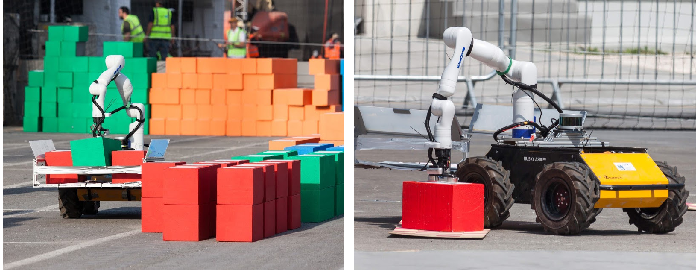
\includegraphics[width=0.45\textwidth]{building.png}\hfill\\[\smallskipamount]
    
    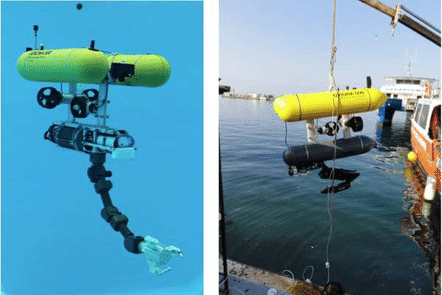
\includegraphics[width=0.22\textwidth]{Girona-500-I-AUV-Left-TRIDENT-configuration-Middle-RAUVI-TRITON-configuration.ppm.png}
    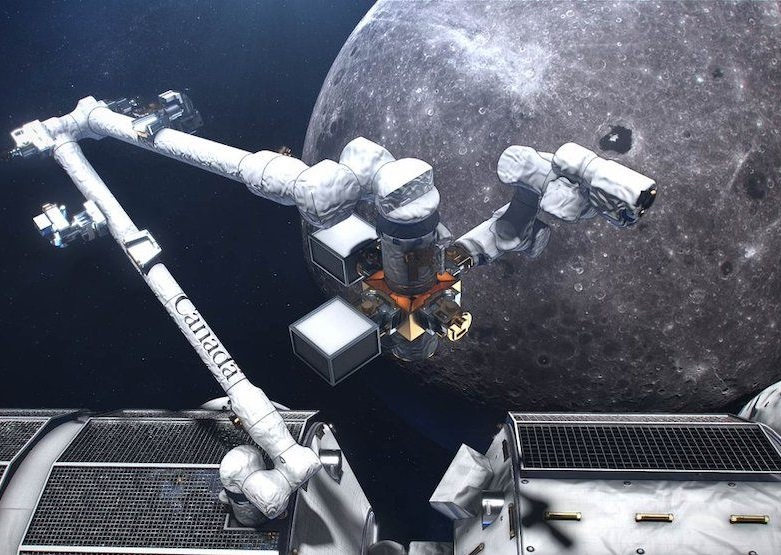
\includegraphics[width=0.22\textwidth]{CanadarmFriend.jpg}
    \caption{Examples of mobile manipulators for construction \cite{vstibinger2021mobile}, underwater recovery missions \cite{ribas2011girona} and in-orbit operations (credit: Canadian Space Agency)}
    \label{fig:bulding}
\end{figure}
These systems are currently used for docking and handling payloads via teleoperation\cite{gibbs2002canada,king2001space, aikenhead1983canadarm}. 
In a space manipulator, the base vehicle has all components of a satellite such as thrusters, Attitude Determination and Control System (ADCS), electronics, telemetry and other subsystems. Its payload is the robotic arm that is deployed once the space manipulator is in the vicinity of a target, in an in-orbit robotic mission.
This article focuses on addressing common problems in the modelling of space-manipulator systems in the manipulator deployment phase. The space manipulator system is mathematically modeled as a multi-body system. The multi-body system consists of a 6 Degree-of-Freedom (DoF) vehicle and a manipulator with a series of joints, most commonly a 3-dof shoulder, a 1-dof elbow, and a 3-dof wrist.
The aim is to analyse the dynamics and enable singularity-free planning and control of the robotic arm from a braked position to reach its end goal. 
The major contributions presented in this article include a complete Lie Group formulation for moving-base multi-body systems with multi-DoF joints and a Lagrange-poincar\'{e} formulation of dynamics for a system on a cartesian product of a Lie Group (vehicle configuration) and a shape space (manipulator's internal states), providing a singularity-free representation of the base dynamics and multi-dof joints and effectively decoupling the external and internal dynamics\cite{park1995lie}. We incorporate an extension of the modeling methods for rigid-body mechanisms to be able to model more general joints the single-dof rotary and prismatic ones. 
This includes all joints for which the configuration space is a Lie group, such as ball joints and 6-dof “free
motion” joints. Common dynamic modelling approaches, such as Hamel equations and Lagrange equations, start from the assumption that the configuration space is isomorphic to $\R^n$. Inspired by the “change of basis” technique used in the constrained force algorithm \cite{}(?), a projection operator is incorporated to utilize exponential coordinates (generated by the Lie algebra) as local Euclidean coordinates. The total relative configuration space of two consecutive bodies in the chain can then be covered by an atlas of local exponential coordinate charts (patches?). The dynamics of a system on a single Lie group can be expressed globally in terms of the group and algebra structures. Locally, the dynamics can be expressed in these coordinates, resulting in explicit and
singularity-free differential equations. The main advantages achieved are a reduced number of state variables and elimination of constraint equations (compared to implicit methods); improved numerical stability due to avoiding singularities; and generally easier integration into model-based control methods such as MPC, RL and computed torque by providing explicit differential equations without constraints. 

The paper is structured as follows:


\section{Related Literature}
\label{chap:MainBackground}


\section{Kinematics of Vehicle-Manipulator Systems on Lie Groups}
\label{math} %\section{Mathematical Background}
%\section{Abstract}
In this section, we provide the kinematics framework that is utilized throughout the article to describe the relative motion of rigid bodies in a moving-base multi-body system based on the Lie Group theory. 
\subsection{Relative Pose and Velocity}
\label{rigidbodykinematics}
%The goal of this section is to provide a formalism for describing motion of a rigid body with respect to a reference coordinate frame or another rigid body. 
Let us consider two rigid bodies in the multi-body system indexed by $i$ and $j$, and attach two orthonormal coordinate frames to them. A relative pose $g^j_i$ between Body $i$ and Body $j$ is a map from the coordinate frame attached to body $i$ to that attached to body $j$ that is isometric and orientation-preserving. The set of all such relative poses forms a smooth manifold that is called the relative configuration manifold and is denoted by $G^j_i$.  %Let us denote the space of all coordinate transformations of Body $i$ by $G^i_i \cong \SE$ and Body $j$ by $G^j_j \cong \SE$. 
Fixing a relative pose, say $\bar{g}^j_i$, there exists an identification of $G^j_i$ by the space of coordinate transformations of Body $i$, $G^i_i$, through left translation , i.e. $G^j_i={\bar{g}^j_i}G^i_i$, and one by $G^j_j$ through right translation, i.e. $G^j_i=G^j_j{\bar{g}^j_i}$. The spaces of coordinate transformations $G^i_i$ and $G^j_j$ are both isomorphic to the Special Euclidean group $\SE$, as Lie groups, and their Lie algebras, respectively denoted by $\g_i^i$ and $\g_j^j$, are isomorphic to $\se$ (the Lie algebra of $\SE$). %$G^j_i$ will then be diffeomorphic to the Special Euclidean Group $\SE$.
%--------------------
%\subsubsection{Relative Velocity of Rigid Bodies} 
\label{difkinrigid}
%For two rigid Bodies $j$ and $i$ , the relative motion of one with respect to the other is a smooth curve $g^j_i(t):[t_0,t_f]\rightarrow G^j_i$ on the relative configuration manifold $G^j_i$. 
An element $g^j_i\in G^j_i$ can be represented via %either represented via the pair $(R^j_i,{}^jp^j_i)$ or alternatively via 
\begin{equation}
    g^j_i=\begin{bmatrix}R^j_i & ^jp^j_i\\\mathbb{O}_{1\times 3} &1\end{bmatrix} 
\end{equation}
where ${R^j_i} \in \SO$ is a ${3 \times 3}$ matrix that describes the orientation of the coordinate frame attached to Body $i$ relative to that attached to Body $j$, and $^jp^j_i \in \R^3$ is the vector of relative linear position between the origins of the same coordinate frames expressed in the frame of Body $j$. $\mathbb{O}_{1\times3}$ is the $1\times 3$ zero matrix.
For a curve $g_i^j(t)\in G_i^j$, the relative velocity of Body $i$ with respect to Body $j$, $\dot{g}^j_i(t)=\frac{d}{dt}g^j_i(t)$, can be observed in the coordinate frame of Body $i$ or Body $j$ via left translation $^i\hat{V}_i^j={g^j_i(t)}^{-1}\dot{g}^j_i(t)\in\mathfrak{g}_i^i$ or right translation $^j\hat{V}_i^j=\dot{g}^j_i(t){g^j_i(t)}^{-1}\in\mathfrak{g}_j^j$, respectively. 
The \textit{hat} operator is the vector space isomorphism between $\R^6$ and $\se$, such that,
\begin{equation}
    \hat{V}:=\begin{bmatrix}\tilde{\omega} & v\\0 & 0\end{bmatrix},
\end{equation}
for every $V=[\omega^T\quad v^T]^T\in \R^6$, where $\tilde{\omega}$ is an element of the Lie algebra of $\SO$, denoted by $\so$, and $v \in \R^3$, corresponding to the angular and linear velocities, respectively. The inverse of the \textit{hat} operator is denoted by \textit{vee}, i.e., $\hat{V}^\vee=V$. The \textit{tilde} operator transforms a vector $\omega\in\R^3$ to a $3 \times 3$ skew-symmetric matrix, such that $\tilde{\omega}p=\omega\times p$, for every $p\in\R^3$. Given the curve $g_i^j(t)$, the two relative velocity matrices are calculated as
\begin{align}
    \begin{split}
   ^i\hat{V}_i^j:&=\begin{bmatrix}({R}^j_i)^T\dot{R}^j_i & (R^j_i)^T{}^j\dot{p}^j_i\\0 & 0\end{bmatrix} \in \g^i_i,\\
    ^j\hat{V}_i^j:&=\begin{bmatrix}\dot{R}^j_i(R^j_i)^T & -\dot{R}^j_i(R^j_i)^T{}^j{p}^j_i+{}^j\dot{p}^j_i\\0 & 0\end{bmatrix} \in \g^j_j.
     \end{split}
     \label{relvel}
\end{align}
%The smooth  manifold $G^j_i$ will then be diffeomorphic to the Special Euclidean Group $\SE$. These two identifications can give rise to two group multiplications on $G^j_i$ that are not necessarily the same, and the fixed pose $\bar{g}^j_i$ acts as the identity element. 
%The rotation part of the coordinate transformation for body $i$ is a member of the Special orthogonal group $R^i_i \in \SO$, and 
%Here, $^iv^i_i$ is a $3 \times 1$ vector belonging to $\R^3$.
%The left and right translation maps by $(g^j_i(t))^{-1}$ are equivalent to left and $L_{g^j_i(t)}$ and right $R_{g^j_i(t)}$ composition maps at point $g^j_i(t)$, respectively. These two representations belong to the Lie algebras $\g^i_i$ and $\g^j_j$.
%Here, $^j\tilde{\omega}^ j_i$ and $^i\tilde{\omega}^ j_i$ are skew-symmetric matrices corresponding to the angular velocity of body $j$ with respect to body $i$ in the coordinate frames attached to body $i$ and body $j$, and the vectors ${}^iv^j_i$ and ${}^jv^j_i$ represent the linear velocity of Body $i$ with respect to Body $j$ expressed in the frames attached to Body $i$ and $j$, respectively.
%Members of the Lie algebra can be identified via a linear mapping between the Lie algebra via the Lie bracket. A Lie Bracket on a matrix lie algebra is defined as the matrix commutator $[A,B]=AB-BA$. This Lie bracket for members of the $so(3)$ lie algebra becomes the cross product $[\tilde{\omega}_1,\tilde{\omega}_2]=\tilde{\omega}_1\times\tilde{\omega}_2$,
%and for a lie algebra isomorphic to $\SE$ takes the form $[(\tilde{\omega}_1,v_1),(\tilde{\omega}_2,v_2)]=(\tilde{\omega}_1\times\tilde{\omega}_2,\tilde{\omega}_1\times v_2-\tilde{\omega}_2\times v_1)$. 
%-----------------------------------
In order to change the coordinate frame of observation, one should use the \textit{Adjoint operator} (for matrix Lie groups):
\begin{equation*}
    ^j\hat{V}_i^j={g^j_i}{}(^i\hat{V}_i^ j)({g^j_i})^{-1}.
\end{equation*}
%of the relative velocities Lie algebra from one coordinate frame to another a conjugate operator is required:
The $6 \times 6$ \textit{Adjoint matrix} which transforms the $\R^6$ representations of the relative velocity vectors from the coordinate frame $i$ to frame $j$ is 
\begin{equation}
    \Ad_{g_i^ j}:=\begin{bmatrix}R_i^ j & (^ j\tilde{p}_i^ j) R_i^ j \\0& R_i^ j\end{bmatrix},
\end{equation}
such that 
\begin{equation}
    ^j{V}_i^j=\Ad_{g^j_i}{}^i{V}_i^j.
    \label{veladj}
\end{equation} 
Based on the Lie bracket of the Lie algebras $\g^i_i$ and $\g^j_j$, we can define the \textit{adjoint operator} $\textbf{ad}_{{}^jV^j_i}(\cdot):=[{^jV^j_i},(\cdot)]$,
where in matrix form
\begin{equation}
\textbf{ad}_{{}^jV^j_i}=\begin{bmatrix}^j\tilde{\omega}_i^{j} & \mathbb{O}_{3\times 3}\\^j\tilde{v}_i^{j} & ^j\tilde{\omega}_i^{j}\end{bmatrix}.
\label{adjlow}
%\textbf{ad}_{{}^j{V}_i^j}
\end{equation}


%%%%%%%%%%%%%%%%%%%
\subsection{Constrained Relative Motion}
%\subsubsection{1-dof Joints} \label{joints}
A joint is a mechanism that restricts the relative motion of body $i$ with respect to body $j$. % to a subset of the tangent bundle of the relative configuration manifold $TG^j_i$. 
In this paper, we consider multi-degree-of-freedom (dof) joints to describe the motion of the base vehicle. We assume that the restricted relative configuration manifold (by an abuse of naming convention) $Q^j_i\subseteq G_i^j$ for a multi-dof joint can be mapped to a $b$-dimensional Lie sub-group of $G^i_i$ or $G^j_j$ through the left or right translation map, using a fixed $\bar{g}^j_i \in Q^j_i$. Let $Q_i^i:=(\bar{g}_i^j)^{-1}Q^j_i\subseteq G_i^i$ be the Lie sub-group associated with $Q_i^j$ whose Lie  sub-algebra is $\mathfrak{q}_i^i\subseteq \g_i^i$.  The dimension $b$ can take values in the set $\{1,2,3,4,6\}$ corresponding to different conjugacy classes of displacement subgroups of $\SE$ \cite{Chhabra2014a}. Such a category of joints can describe the configuration of a wide variety of vehicles, e.g., rovers, drones, spacecraft, rail vehicles, etc., whose motion can include multiple directions. In this paper, we do not use any explicit parametrization of the relative configuration manifold of the base vehicle.
\subsubsection{Parametrization of 1-dof Joints}
We exclusively consider $1$-dof joints for the manipulator. Their restricted relative configuration manifold $Q_i^j$  corresponds to a single admissible direction of relative velocity, where $Q_i^j$ through left (right) translation maps to a 1-parameter Lie subgroup of $G_i^i$ ($G^j_j$). %Here, we exclusively utilize joints where this subset defines a distribution that corresponds to admissible directions of relative velocity of body $i$ with respect to body $j$ at every relative pose. 
%Let us denote the space of all admissible relative poses of body $i$ with respect to body $j$ considering the joint constraints by $Q^j_i$, and hereinafter call it the relative configuration manifold, by an abuse of naming convention. The dimension of $Q^j_i$ is named the degree-of-freedom (dof) of the joint. 
%The appropriate parameterization of $Q^j_i$ is one of the critical practical problems in mechanics, due to its influence on the efficiency of dynamical analysis and control of multi-body systems. 
%Let us fix $\bar{g}^j_i \in Q^j_i$ and 
%We can define $Q_j$ by the left composition of $Q^j_i$ by the fixed $(\bar{g}^j_i)^{-1}$, then any element in a local neighborhood of $\bar{g}^j_i$ can be parametrized by a local coordinate chart for a neighborhood of the identity element $e_j \in Q_j$. A velocity vector $V^j_i \in T_{g^j_i}Q^j_i$ at an arbitrary relative pose $g^j_i$ can be consequently identified with an element of the induced coordinate chart for the tangent bundle. 
% screw theory
%Chasles' theorem \cite{whittaker1937treatise} states that every rigid body transformation can be achieved by a \textit{screw motion}, %from any initial relative pose $\bar{g}^j_i$, an arbitrary relative configuration $g^j_i \in G^j_i$ of a rigid body can be achieved by a .
%Here, a set of joint parameters called screw joint parameters is introduced. If the relative velocity vector field of two bodies is independent of time, the respective relative motion can be called relative screw motion. The naming stems from an interpretation of  
The exponential map of the Lie group $\SE$ is a diffeomorphism from a local neighborhood of the origin of the Lie algebra $\se$ to a local neighborhood of the identity element of $\SE$, which geometrically corresponds to a simultaneous rotation about and translation along a fixed vector in $\R^3$, where the ratio of translation to rotation is constant.  %, which provides a local coordinate chart to parametrize $Q^j_i$\cite{Chhabra2014a}. %Using the exponential map, the 1-dof revolute, prismatic and helical joints can be (globally) parameterized via 1-dimensional sub-spaces of $\se$ that provide multiple coverings of their configuration manifolds \cite{Chhabra2014}. 
The right (left) translation via a fixed relative configuration $\bar{g}^j_i\in Q_i^j$ along with the group exponential map of $G^j_j$ ($G_i^i$), induced by $\SE$, introduces a parametrization of the relative configuration manifold $Q_i^j$ of 1-dof joints through  
%The screw joint parameters %$q_i \in \R^n$, %physically corresponding to the initial classic joint speeds for a screw motion on the corresponding relative configuration manifold,
%enable the representation of every rigid motion (and by extension a relative configuration $g^j_i$, through left or right translation via a fixed relative configuration) via the group exponential map of an element  as: % that  By incorporating the product of exponentials formula, the transformation matrix $g^j_i\in \SE$ (the action of the group element $g^j_i$ on the point $q_j \in \R $) can be broken into two parts: 
\begin{align}
       g^j_i(q)=\exp(^j\hat{\xi}^j_iq)\bar{g}^j_i=e^{^j\hat{\xi}^j_iq}\bar{g}^j_i,\label{twistform1}\\ g^j_i(q)=\bar{g}^j_i{}\exp(^i\hat{\xi}^j_iq)=\bar{g}^j_i{} e^{^i\hat{\xi}^j_iq} ,
\end{align}
where $q$ is the joint parameter, corresponding to the amount of rotation and/or translation. The \textit{twist vector} $^j\xi_i^j$ ($^i\xi_i^j$) corresponds to the axis of the relative screw motion observed from the coordinate frame of Body $j$ (Body $i$). In this paper, we only work with the right translation map for joint parameterization, i.e., \eqref{twistform1}. The exponential term gives the required transformation to go from the fixed relative configuration $\bar{g}^j_i$ to any relative configuration of the joint. %$\hat{\xi}^i_i$ is called the twist matrix corresponding to screw motion by the $i^{th}$ joint in the system and $q_i$ is the screw joint parameter corresponding to the motion along the allowed DoF of that joint. 
The twist vector and twist matrix for different 1-dof joints can be calculated from the following equations: 
%of $i$th joint in an open-chain multi-body system, defined rigorously in Section \ref{diffkin}, can be geometrically calculated from
\begin{equation}
    ^j\xi^j_i=\begin{bmatrix}^j\varpi_i^j \\^j\nu^j_i\end{bmatrix} \quad \& \quad ^j\hat{\xi}^j_i=\begin{bmatrix}^j\tilde{\varpi}_i^j  & ^j\nu^j_i \\0 & 1\end{bmatrix}, \label{twist1}
\end{equation}
%where, for a 1-DoF joint, $\omega_i^j$ is the axis of rotation of the joint and $^jp^j_i$ is the the position vector of the origin of that joint at the initial configuration. The $4\times4$ matrix representation $\hat{\xi}_i$ belongs to $\SE$ (NO!!! where has this come from??). 
where $^j\varpi_i^j$ represents the axis of rotation of the joint observed from Body $j$, which for prismatic joints becomes zero. For prismatic joints $^j\nu^j_i$ is a unit vector in the direction of translation observed from Body $j$, for revolute joints $^j\nu^j_i= -{}^j\varpi_i^j \times {}^j\rho_i^j$, and for helical joints $^j\nu^j_i= -{}^j\varpi_i^j \times {}^j\rho_i^j+\mathfrak{p}^j_i{}^j\omega^j_i$. Here, $\mathfrak{p}^j_i$ is the pitch of the helical joint, and $^j\rho^j_i$ is the position vector of a point on the joint axis observed from Body $j$, commonly considered to be the position of the joint.
%These two representations of the twist can be transformed into eachother via the \textit{wedge} and \textit{vee} operators
%\begin{equation}
%    {\xi^j_i}^{\wedge}=\hat{\xi}^j_i \quad \& \quad {\hat{\xi}^j_i}^{\vee}=\xi^j_i.
%\end{equation}
The use of Rodrigues' formula provides a means for calculating the exponential term in the parameterization of 1-dof joints \cite{murray1994mathematical}. Let $\hat{\xi}\in\se$ such that $\xi=[\varpi^T\quad \nu^T]^T$:
\begin{equation}
\begin{split}
    e^{\hat{\xi}q}=\begin{bmatrix}I & \nu q \\ 0 & 1\end{bmatrix}, &\quad |\varpi|=0\\
    e^{\hat{\xi}q}=\begin{bmatrix} e^{\tilde{\varpi}q}& (I-e^{\tilde{\varpi}q})(\tilde{\varpi} \time {}v)+\varpi {\varpi}^T \nu q \\0 &1\end{bmatrix}, &\quad |\varpi| = 1
    \end{split}
\end{equation}
where the exponential term $e^{\tilde{\varpi}q}=R \in \SO$ corresponds to the rotation part of a transformation, found from Rodrigues' formula ($|\varpi|=1$) \cite{murray1994mathematical}:
\begin{equation}
    e^{\tilde{\varpi}q}=I+\tilde{\varpi}\sin(q)+ \tilde{\varpi}^2\big(1-\cos (q)\big),
\end{equation}
%with $\omega^j_i=^i\omega^j_i$ or $\omega^j_i=^j\omega^j_i$ being the axis of rotation of the joint.
%expand $ e^{\hat{\omega}^j_iq_i}$.
and the term $(I-e^{\hat{\varpi}q})(\varpi \time {}\nu)+\varpi {\varpi}^T \nu q$ represents the linear translation. 

\subsection{Vehicle-Manipulator System Kinematics}\label{kinematics}
A vehicle-manipulator system moving with respect to an inertial frame $\mathcal{I}$ can be modelled as an open-chain multi-body system. To avoid complexity in notation, we only study a single-branch arm, i.e., a serial-link multi-body system. The extension of this work to multi-branch manipulators is straightforward. A serial-link multi-body system is a collection of $n+1$ bodies indexed by $\{0,1,\cdots, n\}$, where $0$ corresponds to the base vehicle, and $n+1$ joints between the consecutive bodies labeled by the succeeding body's index. %The coordinate frame of the base vehicle $\B$ is indexed by $0$. 
We attach reference frames to each link at its preceding joint and express its inertial parameters in these local frames. %The manipulator links are indexed by the set $\{1,\cdots,n\}$, where $n$ corresponds to the end-effector and is interchangeably referred to as $ee$.
Let $Q^I_0$ denote the $b$-dimensional relative configuration manifold of the base vehicle with respect to the inertial frame $\mathcal{I}$. The relative configuration manifold $Q^{I}_0$ is identified via a Lie group through the right translation by a fixed relative pose $\bar{g}^I_0{} \in Q_0^I$. %The developed formulation of this article is applicable to any moving-base manipulator system where the motion of the base can be identified via a Lie group (e.g. planar motion, ball joint, rail, or $\SE$ as in drones, aircraft and vehicles). 
We have chosen the initial relative configuration of in a robotic operation as the aforementioned fixed pose $\bar{g}^I_0{}$. To avoid singularities due to parameterization, we will directly work with members of $Q^I_0$ when formulating the kinematics and dynamics of the system. %This treatment of the base configuration avoids all forms of kinematic singularities in their entirety.  %(?) $D^o_b$ and $D^I_b$ are therefore 6-DoF spaces. 
Since we only consider 1-dof joints for the manipulator system, the relative configuration manifolds $Q^{i-1}_i $ $(i=1, \cdots, n) $ of consecutive manipulator links, are parameterized using the exponential map: 
\begin{align}
g_i^{i-1}=\exp{({}^{i-1}\hat{\xi}^{i-1}_iq_i)}\bar{g}^{i-1}_i\in Q_i^{i-1}\label{expparam}
\end{align}
where ${}^{i-1}\hat{\xi}^{i-1}_i$ is the joint axis defined in \eqref{twist1}, $q_i$ is the joint parameter, and $\bar{g}^{i-1}_i$ belongs to $Q^{i-1}_i$. %Here, we only consider one-parameter sub-groups of $\SE$ to describe the relative configuration manifolds of the manipulator joints, which correspond to 1-dof rotary, prismatic and helical joints. %Therefore, an exponential formulation of robot joint motion is utilized to form the relative position  of each manipulator body $i$ with respect to its preceding body in the chain $j$ based on the joint parameter $q_i$. %The manipulator joints are modeled as 1-DoF rotary and prismatic joints. so their $D_i^j$ is a 1-DoF space. 
Let $Q_\mathfrak{m}$ denote the $n$-dimensional configuration manifold of the manipulator. An element $q_\mathfrak{m} \in Q_\mathfrak{m}$ consists of a set of joint parameters of the manipulator $[q_1,\cdots,q_n]^T$. We also denote the $(b+n)$-dimensional configuration manifold of the vehicle manipulator by $Q:=Q^I_0 \times Q_\mathfrak{m}$. %An element $q \in Q$ is a tuple $\{g_0^I,q_m\}$ consisting of pose of the base vehicle and joint parameters of the manipulator.%The configuration manifold $Q_\mathfrak{m}$ includes all possible values of the joint parameters.
\subsubsection{Forward Kinematics}
\label{forwardkinematics}
%A configuration of the moving-base open-chain multi-body system is defined as the collection of relative configurations of the individual bodies $q:=(g^I_0 ,q_\mathfrak{m}) \in Q^I_0 \times Q_\mathfrak{m}$.
Given a base configuration $g^I_0 \in Q_0^I$, and a set of joint angles $q_\mathfrak{m} \in Q_\mathfrak{m}$,  % and the geometry of the vehicle, arm and the orbits, 
the \textit{Forward Kinematics} (FK) is a smooth map from $q:=(g^I_0 ,q_\mathfrak{m}) \in Q$ to the relative pose of a body in the chain with respect to a chosen frame. For the purposes of this study, this reference frame can be the base vehicle's or the inertial frame.
The pose of Body $i$ with respect to the inertial frame is formulated by:
\begin{equation}
    g^I_{i}(g^I_0, q_\mathfrak{m})=g^I_{0}g^0_{i}(q_\mathfrak{m}),
\end{equation}
where the base vehicle's configuration is
%\begin{equation}
%    g^I_o(q_o)=e^{\hat{\xi}_{o_\theta}q_{o_\theta}}e^{\hat{\xi}_{o_r}q_{o_r}}g^I_o(0)
%\end{equation}
\begin{equation}
    g^I_0 =\begin{bmatrix}R^I_0 & ^Ip^I_0\\0&1\end{bmatrix},
\end{equation}
%For simplicity, $^Ip^I_0$ and $R^I_0$ are the position of the center of mass of the base vehicle and its orientation with respect to the inertial frame expressed in the same frame. %The generalized exponential formula for the Forward Kinematics map corresponding to the manipulator can be formulated as
and based on \eqref{expparam}, the product of exponentials formula \cite{murray1994mathematical} leads to
\begin{equation}
    g^0_i(q_\mathfrak{m})=e^{\hat{\xi}_{1}q_{1}}...e^{\hat{\xi}_{i}q_{i}}\bar{g}^0_{i}.
\end{equation}
%\begin{equation}
%    g^I_i(g^I_0, q_\mathfrak{m})=g^I_0e^{\hat{\xi}_{1}q_{1}}...e^{\hat{\xi}_{i}q_{i}}\bar{g}^0_{i},
%\end{equation}the configuration of body $i$ with respect to the vehicle frame represented in the same frame via the use of generalized exponential formula is:
Here, $\bar{g}^0_i=\bar{g}^0_1\cdots \bar{g}^{i-1}_i$ is a fixed relative pose of Body $i$ with respect to the vehicle (commonly chosen to be the initial pose), and the new notation
\begin{equation}
  {\xi}_i:= \Ad_{\bar{g}^0_{i-1}}{}^{i-1}{\xi}^{i-1}_i\in(\mathfrak{g}_0^0)^\vee, \label{twist}
\end{equation}
represent the manipulator's joints' twist matrices expressed in the base vehicle's initial coordinate frame. % calculated rigorously in Section \ref{diffkin}:
%\begin{equation}
%    ^{\bar{0}}\hat{V}^{i-1}_i=\big(\Ad_{\bar{g}^0_{i-1}}{}^{i-1}\hat{V}_{i}^{i-1}\big)=^{\bar{0}}\hat{\xi}^{i-1}_i\dot{q}_i=\hat{\xi}_i\dot{q}_i
 %   \label{twist}
%\end{equation}
In order to calculate the kinetic energy of the system, we further require to find the pose of the center of mass of Body $i$ with respect to $\mathcal{I}$, denoted by $g^I_{cm,i}$, as:
\begin{equation}
    g^I_{cm,i}=g^I_i\,\bar{g}^i_{cm,i}=g^I_0e^{\hat{\xi}_{1}q_{1}}...e^{\hat{\xi}_{i}q_{i}}\bar{g}^0_{cm,i},
\end{equation}
where $\bar{g}^i_{cm,i}$ and $\bar{g}^0_{cm,i}$ are the constant pose of the coordinate frame attached to the center of mass of Body $i$ with respect to the corresponding joint coordinate frame and the base vehicle's initial frame, respectively.

\begin{example}{ \textit{Planar Vehicle:}}
The forward kinematics of a manipulator mounted on a planar vehicle is formulated in the following section. The vehicle can be considered as a 3-dof moving joint as can be seen in Figure \ref{fig:planar}. The multi-body system consists of three bodies, one base joint and two single-dof perpendicular manipulator joints.

\begin{figure}[htbp]
\begin{center}

\begin{tikzpicture}[scale=0.4]
% ground
\draw[fill=gray!4, fill opacity=1] (7.5,-1,9) -- (7.5,-1,-4) -- (-5,-1,-4) -- (-5,-1,9) -- cycle; 

% Wheel back  
        \node[cylinder, draw, cylinder body fill = gray, minimum width=30, fill=gray!120] (c) at (-3,-1.3,-0.3) {};

% Orbit Axes
        \coordinate (O) at (0,0,0) node[below right]{$B$};
        \draw[axis] (O) -- ++(1.5,0,0) node[right] {$x$};
        \draw[axis] (O) -- ++(0,1.5,0) node[above right] {$y$};
        \draw[axis] (O) -- ++(0,0,1.5) node[above] {$z$};

%Base Sat

    \draw[fill=gray!35, fill opacity=1] (-2,-2,2) -- (-2,0.7,2) -- (2,0.7,2) -- (2,-2,2) -- cycle; 
    \draw[fill=gray!70, fill opacity=1] (2,0.7,2) -- (2,0.7,-2) -- (2,-2,-2) -- (2,-2,2) -- cycle; 
    \draw[fill=gray!4, fill opacity=1] (2,0.7,2) -- (2,0.7,-2) -- (-2,0.7,-2) -- (-2,0.7,2) -- cycle; 
        
% joint 1        
        \draw[fill=gray!50] (0,0,2) circle (0.4); 
        \draw[fill=gray!20] (O,0,2.1) circle (0.4);
        %\filldraw[ball color=white] (0,0,2.1) circle (0.3);
        \draw[fill=gray!15] (O,0,2.4) circle (0.2);
    \fill[fill=gray!15] (0,0.1,2.3) -- (0,-0.1,2.3) -- ++(0,0,3) -- (0,0.1,5.3) -- cycle;
    \draw (0,0.1,2.3) -- ++(0,0,3);
    \draw (0,-0.1,2.3) -- ++(0,0,3) node[right,midway];
    
     \node[cylinder, draw, cylinder body fill = white!50, minimum width=11, fill=grey!7] (c) at (-0.2,0,2) {};

% Link 1
    \draw[fill=gray!15] (O,0,2.4) circle (0.2);
    \fill[fill=gray!15] (-0.175,0.1,2.3) -- (0.175,-0.1,2.3) -- ++(0,0,3) -- (-0.175,0.1,5.3) -- cycle;
    \draw (-0.175,0.1,2.3) -- ++(0,0,3);
    \draw (0.175,-0.1,2.3) -- ++(0,0,3) node[right,midway];

% joint 2
        \draw (-0.2,0.4,5.2) -- (0.2,0.4,5.2) -- (0.2,-0.4,5.2) -- (-0.2,-0.4,5.2) -- cycle;
        \draw[fill=gray!10] (-0.2,0,5.2) ellipse (0.166 and 0.4);
        \fill[fill=gray!10] (-0.2,0.4,5.2) -- (0.2,0.4,5.2) -- (0.2,-0.4,5.2) -- (-0.2,-0.4,5.2) -- cycle;
        \draw[fill=gray!50] (0.2,0,5.2) ellipse (0.166 and 0.4);

% joint 3
        \draw (0.4,-0.2,5.2) -- (0.4,0.2,5.2) -- (-0.4,0.2,5.2) -- (-0.4,-0.2,5.2) -- cycle;
        \draw[fill=gray!40] (0,-0.2,5.2) ellipse (0.4 and 0.266);
        \fill[fill=gray!40] (0.4,-0.2,5.2) -- (0.4,0.2,5.2) -- (-0.4,0.2,5.2) -- (-0.4,-0.2,5.2) -- cycle;
        \draw[fill=gray!10] (0,0.2,5.2) ellipse (0.4 and 0.266);
        
% Link 2
    \draw[fill=gray!10] (O,0,5.6) circle (0.2);
    \fill[fill=gray!10] (-0.175,0.1,5.5) -- (0.175,-0.1,5.5) -- ++(0,0,3) -- (-0.175,0.1,8.5) -- cycle;
    \draw (-0.175,0.1,5.5) -- ++(0,0,3);
    \draw (0.175,-0.1,5.5) -- ++(0,0,3) node[right,midway];


        
% end-effector
        
    \draw[fill=gray!130] (-0.4,-0.4,8.7) -- (-0.4,0.4,8.7) -- (0.4,0.4,8.7) -- (0.4,-0.4,8.7) -- cycle; 
    \draw[fill=gray!170] (0.4,0.4,8.7) -- (0.4,0.4,8) -- (0.4,-0.4,8) -- (0.4,-0.4,8.7) node[right]{End-Effector} -- cycle; 
    \draw[fill=gray!100] (0.4,0.4,8.7) -- (0.4,0.4,8) -- (-0.4,0.4,8) -- (-0.4,0.4,8.7) -- cycle;
    
    \draw[fill=gray!130] (-0.4,-0.4,8.7) -- (-0.4,0.4,8.7) -- (-0.1,0.4,9.1) -- (-0.1,-0.4,9.1) -- cycle;
    \draw[fill=gray!150] (-0.1,-0.4,8.7) -- (-0.1,0.4,8.7) -- (-0.1,0.4,9.1) -- (-0.1,-0.4,9.1) -- cycle;
    
    \draw[fill=gray!100] (0.1,0.4,9.1) -- (0.1,0.4,8.7) -- (0.4,0.4,8.7)-- cycle;
    \draw[fill=gray!160] (0.1,-0.4,9.1) -- (0.1,0.4,9.1) -- (0.4,0.4,8.7) -- (0.4,-0.4,8.7) -- cycle;
    
% Wheels   
        \node[cylinder, aspect=1.2, draw, fill=gray!120, minimum width=30] (c) at (2,-1.2,-0.3) {};

% Axes
    \coordinate (1) at (0,0,2.1);
        \draw[axis] (1) -- ++(0.85,0,0) node[right] {$\varpi_1$};
        \draw[axis] (0.2,0.4,5.4) -- ++(0,0.85,0)  node[left] {$\varpi_2$};

% Labels

% Angles
    
\end{tikzpicture}
\end{center}
\caption{Planar Vehicle-Manipulator System}
\label{fig:planar}
\end{figure}
\end{example}
The fixed initial absolute configuration of the spacecraft joint which is the same as its center of mass is
\begin{equation*}
    \bar{g}^I_0=\bar{g}^I_{0,cm}=\begin{bmatrix}1 &0 &0&0 \\0 &1 &0& 0\\0 & 0& 1&h_0 \\0 & 0 & 0 & 1
    \end{bmatrix}
\end{equation*}
Thus we identify the elements of the relative configuration manifold of the base rover to the inertia, which is a 3-dof planar joint motion, by
\begin{equation}
    G^I_0=\Bigg\{\begin{bmatrix}
    R_{Z_{3 \times 3}} & \begin{bmatrix}
    x \\ y \\ 0
    \end{bmatrix}\\ \begin{bmatrix}
    0 & 0 & 0
    \end{bmatrix} & 1
    \end{bmatrix}\Bigg| R_Z \in \textbf{SO}(1),x,y\in\mathbb{R} \Bigg\},
\end{equation}
where
\begin{equation}
    R_Z(\theta_z)=\begin{bmatrix}
    1 & 0 & 0\\0 &cos\theta_z & -sin\theta_z\\0 & sin\theta_z & cos\theta_z
    \end{bmatrix}.
\end{equation}
The first arm link is attached to the vehicle at $^0\rho^0_1=\begin{bmatrix}0 & 0 &l_1\end{bmatrix}^T$, and its corresponding revolute joint generates rotation about $^0\varpi^0_1=\begin{bmatrix} 1 & 0 & 0\end{bmatrix}^T$, resulting in a twist of the form:
\begin{equation*}
    \hat{\xi}_1={}^0\hat{\xi}^0_1=\begin{bmatrix}0 &0 &0&0 \\0 &0 &-1& l_0\\0 & 1& 0&0 \\0 & 0 & 0 & 1
    \end{bmatrix}
\end{equation*}
The fixed initial absolute/relative configuration of the first joint is
\begin{equation*}
    \bar{g}^0_1=\begin{bmatrix}1 &0 &0&0 \\0 &1 &0& l_0\\0 & 0& 1&0 \\0 & 0 & 0 & 1
    \end{bmatrix} \quad \& \quad  \bar{g}^I_1=\begin{bmatrix}1 &0 &0&0 \\0 &1 &0& l_0\\0 & 0& 1&0 \\0 & 0 & 0 & 1
    \end{bmatrix}
\end{equation*}
The resulting initial relative and absolute configurations of the center of mass of the first link are
\begin{equation*}
    \bar{g}^1_{1,cm}=\begin{bmatrix}1 &0 &0&0 \\0 &1 &0& \frac{l_1}{2}\\0 & 0& 1&0 \\0 & 0 & 0 & 1
    \end{bmatrix} \quad \& \quad  \bar{g}^I_{1,cm}=\begin{bmatrix}1 &0 &0&0 \\0 &1 &0& l_0+\frac{l_1}{2}\\0 & 0& 1&0 \\0 & 0 & 0 & 1
    \end{bmatrix}
\end{equation*}
The second link is attached to the first at the fixed relative linear position $^1\rho^1_2=\begin{bmatrix}0 & 0 &l_1\end{bmatrix}^T$ in the first joint's frame, which corresponds to a $ ^0\bar{\rho}^0_2=\begin{bmatrix}0 & 0 &l_0+l_1\end{bmatrix}^T$ absolute \textit{initial} position and its corresponding revolute joint generates rotation about $^0\varpi^0_2=\begin{bmatrix} 0 & 1 & 0\end{bmatrix}^T$, resulting in a twist of the form:
\begin{equation*}
    \hat{\xi}_2=\Ad_{\bar{g}^0_{1}}{}^{1}{\xi}^{1}_2=\begin{bmatrix}0 &0 &0&-l_0-l_1 \\0 &0 &-1& 0\\0 & 1& 0&0 \\0 & 0 & 0 & 1
    \end{bmatrix}
\end{equation*}
The initial relative and absolute configurations of the second joint are
\begin{equation*}
    \bar{g}^1_2=\begin{bmatrix}1 &0 &0&0 \\0 &1 &0& l_1\\0 & 0& 1&0 \\0 & 0 & 0 & 1
    \end{bmatrix} \quad \& \quad \bar{g}^I_2=\begin{bmatrix}1 &0 &0&0 \\0 &1 &0& l_0+l_1\\0 & 0& 1&0 \\0 & 0 & 0 & 1
    \end{bmatrix}
\end{equation*}
The resulting initial relative and absolute configurations of the center of mass of the second link are
\begin{equation*}
    \bar{g}^2_{2,cm}=\begin{bmatrix}1 &0 &0&0 \\0 &1 &0& \frac{l_2}{2}\\0 & 0& 1&0 \\0 & 0 & 0 & 1
    \end{bmatrix}\& \bar{g}^I_{2,cm}=\begin{bmatrix}1 &0 &0&0 \\0 &1 &0& l_0+l_1+\frac{l_2}{2}\\0 & 0& 1&0 \\0 & 0 & 0 & 1
    \end{bmatrix}
\end{equation*}
Thus we identify the elements of the relative configuration manifold of the base spacecraft to the inertia, which is a 6-dof free joint motion, by
\begin{equation}
    Q^I_0=\Bigg\{g^I_0=\begin{bmatrix}
    R_{3 \times 3} & \begin{bmatrix}
    x \\ y \\ z
    \end{bmatrix}\\ \begin{bmatrix}
    0 & 0 & 0
    \end{bmatrix} & 1
    \end{bmatrix}\Bigg| R \in \SO,x,y,z\in\mathbb{R} \Bigg\}.
\end{equation}
The first manipulator joint is a 1-dof revolute joint between spacecraft and link 1, and its corresponding  constrained relative configuration manifold $Q^0_1$, identified via right translation of $G^0_1$ by $\bar{g}^0_1$, is given by
\begin{equation}
    Q^0_1=\Bigg\{g^0_1=
    \resizebox{0.5\hsize}{!}{\begin{bmatrix}
    1 & 0 & 0 & 0\\0 &\cos q_1 & -\sin q_1 & l_1\sin q_1\\0 & \sin q_1  & \cos q_1 & l_1(1-\cos q_1)\\  0 & 0 & 0 & 1
    \end{bmatrix}}\bar{g}^0_1\Bigg| q_1 \in \mathbb{S} \Bigg\}.
\end{equation}
The second manipulator joint is a 1-dof revolute joint between link 1 and link 2,  and its corresponding  constrained relative configuration manifold $Q^1_2$, identified via right translation of $G^1_2$ by $\bar{g}^1_2$, is given by
\begin{equation}
    Q^1_2=\Bigg\{g^1_2=
    \resizebox{0.5\hsize}{!}{\begin{bmatrix}
    \cos q_2  & 0 & \sin q_2 & -\sin q_2(l_1+l_2)\\0 & 1& 0 & 0\\-\sin q_2 & 0 & \cos q_2 & (1-\cos q_2)(l_1+l_2)\\  0 & 0 & 0 & 1
    \end{bmatrix}}\bar{g}^1_2\Bigg| q_2 \in \mathbb{S} \Bigg\}.
\end{equation}

\begin{example}{\textit{Spacecraft-Manipulator:}}
In this section, the kinematic analysis of a space manipulator consisting of a 2-dof manipulator mounted on a free-floating vehicle (spacecraft) is presented. The motion of the base spacecraft is equivalent to a 6-dof free-moving joint as seen in \ref{fig:planar}. The attitude of a spacecraft is commonly described via Euler parameters or quaternions, motivated by the need to push the singularities in their representation to less occuring values. We will use a Lie group representation of the base joint instead, which enables an entirely non-singular treatment. The multi-body system consists of two other single-dof joint on top of the mentioned base joint, which represent the perpendicular manipulator joints.

\begin{figure}[htbp]
\begin{center}

\begin{tikzpicture}[trimetric,scale=0.5]


% Orbit Axes
        \coordinate (O) at (0,0,0) node[below right]{$B$};
        \draw[axis] (O) -- ++(1.5,0,0) node[right] {$x$};
        \draw[axis] (O) -- ++(0,1.5,0) node[above right] {$y$};
        \draw[axis] (O) -- ++(0,0,1.5) node[above] {$z$};
%Base Sat

        
    \draw[fill=gray!35, fill opacity=0.5] (-2,-2,2) -- (-2,2,2) -- (2,2,2) -- (2,-2,2) -- cycle; 
    \draw[fill=gray!70, fill opacity=0.5] (2,2,2) -- (2,2,-2) -- (2,-2,-2) -- (2,-2,2) -- cycle; 
    \draw[fill=gray!4, fill opacity=0.5] (2,2,2) -- (2,2,-2) -- (-2,2,-2) -- (-2,2,2) -- cycle; 
        
% joint 1        
        %\draw[fill=gray!50] (0,0,2) circle (0.4); 
        \draw[fill=gray!20] (O,0,2.1) circle (0.4);
        %\filldraw[ball color=white] (0,0,2.1) circle (0.3);
        \draw[semithick] (0.2,0,2.1) arc (90:165.270:1);

% joint 2
        \draw (O,0,2.1) -- (0.2,0.4,5.2) -- (O.4,0,2.1) -- (O,-0.4,2.1) -- cycle;
        \draw[fill=gray!10] (-0.2,0,5.2) ellipse (0.166 and 0.4);
        \fill[fill=gray!10] (-0.2,0.4,5.2) -- (0.2,0.4,5.2) -- (0.2,-0.4,5.2) -- (-0.2,-0.4,5.2) -- cycle;
        \draw[fill=gray!50] (0.2,0,5.2) ellipse (0.166 and 0.4);

% Link 1
    \draw[fill=gray!15] (O,0,2.4) circle (0.2);
    \fill[fill=gray!15] (-0.175,0.1,2.3) -- (0.175,-0.1,2.3) -- ++(0,0,3) -- (-0.175,0.1,5.3) -- cycle;
    \draw (-0.175,0.1,2.3) -- ++(0,0,3);
    \draw (0.175,-0.1,2.3) -- ++(0,0,3) node[right,midway];


   
% joint 3
        \draw (0.4,-0.2,5.2) -- (0.4,0.2,5.2) -- (-0.4,0.2,5.2) -- (-0.4,-0.2,5.2) -- cycle;
        \draw[fill=gray!40] (0,-0.2,5.2) ellipse (0.4 and 0.266);
        \fill[fill=gray!40] (0.4,-0.2,5.2) -- (0.4,0.2,5.2) -- (-0.4,0.2,5.2) -- (-0.4,-0.2,5.2) -- cycle;
        \draw[fill=gray!10] (0,0.2,5.2) ellipse (0.4 and 0.266);
        
% Link 2
    \draw[fill=gray!10] (O,0,5.6) circle (0.2);
    \fill[fill=gray!10] (-0.175,0.1,5.5) -- (0.175,-0.1,5.5) -- ++(0,0,3) -- (-0.175,0.1,8.5) -- cycle;
    \draw (-0.175,0.1,5.5) -- ++(0,0,3);
    \draw (0.175,-0.1,5.5) -- ++(0,0,3) node[right,midway];




% end-effector
        
    \draw[fill=gray!130] (-0.4,-0.4,8.7) -- (-0.4,0.4,8.7) -- (0.4,0.4,8.7) -- (0.4,-0.4,8.7) -- cycle; 
    \draw[fill=gray!170] (0.4,0.4,8.7) -- (0.4,0.4,8) -- (0.4,-0.4,8) -- (0.4,-0.4,8.7) node[below right]{End-Effector} -- cycle; 
    \draw[fill=gray!100] (0.4,0.4,8.7) -- (0.4,0.4,8) -- (-0.4,0.4,8) -- (-0.4,0.4,8.7) -- cycle;
    
    \draw[fill=gray!130] (-0.4,-0.4,8.7) -- (-0.4,0.4,8.7) -- (-0.1,0.4,9.1) -- (-0.1,-0.4,9.1) -- cycle;
    \draw[fill=gray!150] (-0.1,-0.4,8.7) -- (-0.1,0.4,8.7) -- (-0.1,0.4,9.1) -- (-0.1,-0.4,9.1) -- cycle;
    
    \draw[fill=gray!100] (0.1,0.4,9.1) -- (0.1,0.4,8.7) -- (0.4,0.4,8.7)-- cycle;
    \draw[fill=gray!160] (0.1,-0.4,9.1) -- (0.1,0.4,9.1) -- (0.4,0.4,8.7) -- (0.4,-0.4,8.7) -- cycle;

% Axes
    \coordinate (1) at (0,0,2.1);
        \draw[axis] (1) -- ++(0.85,0,0) node[right] {$\varpi_1$};
        \draw[axis] (0.2,0.4,5.4) -- ++(0,0.85,0)  node[left] {$\varpi_2$};

% Labels

% Angles
    
\end{tikzpicture}
\end{center}
\caption{Satellite Manipulator System}
\label{fig:my_label}
\end{figure}
The fixed initial absolute configuration of the spacecraft joint which is the same as its center of mass is
\begin{equation*}
    \bar{g}^I_0=\bar{g}^I_{0,cm}=\begin{bmatrix}1 &0 &0&0 \\0 &1 &0& 0\\0 & 0& 1&0 \\0 & 0 & 0 & 1
    \end{bmatrix}
\end{equation*}

The first arm link is attached to the spacecraft at $^0\rho^0_1=\begin{bmatrix}0 & 0 &l_1\end{bmatrix}^T$, and its corresponding revolute joint generates rotation about $^0\varpi^0_1=\begin{bmatrix} 1 & 0 & 0\end{bmatrix}^T$, resulting in a twist of the form:
\begin{equation*}
    \hat{\xi}_1={}^0\hat{\xi}^0_1=\begin{bmatrix}0 &0 &0&0 \\0 &0 &-1& l_0\\0 & 1& 0&0 \\0 & 0 & 0 & 1
    \end{bmatrix}
\end{equation*}
The fixed initial absolute/relative configuration of the first joint is
\begin{equation*}
    \bar{g}^0_1=\begin{bmatrix}1 &0 &0&0 \\0 &1 &0& 0\\0 & 0& 1& l_0 \\0 & 0 & 0 & 1
    \end{bmatrix} \quad \& \quad  \bar{g}^I_1=\begin{bmatrix}1 &0 &0&0 \\0 &1 &0& 0\\0 & 0& 1&l_0 \\0 & 0 & 0 & 1
    \end{bmatrix}
\end{equation*}
The resulting initial relative and absolute configurations of the center of mass of the first link are
\begin{equation*}
    \bar{g}^1_{1,cm}=\begin{bmatrix}1 &0 &0&0 \\0 &1 &0& \frac{l_1}{2}\\0 & 0& 1&0 \\0 & 0 & 0 & 1
    \end{bmatrix} \quad \& \quad  \bar{g}^I_{1,cm}=\begin{bmatrix}1 &0 &0&0 \\0 &1 &0& l_0+\frac{l_1}{2}\\0 & 0& 1&0 \\0 & 0 & 0 & 1
    \end{bmatrix}
\end{equation*}
The second link is attached to the first at the fixed relative linear position $^1\rho^1_2=\begin{bmatrix}0 & 0 &l_1\end{bmatrix}^T$ in the first joint's frame, which corresponds to a $ ^0\bar{\rho}^0_2=\begin{bmatrix}0 & 0 &l_0+l_1\end{bmatrix}^T$ absolute \textit{initial} position and its corresponding revolute joint generates rotation about $^0\varpi^0_2=\begin{bmatrix} 0 & 1 & 0\end{bmatrix}^T$, resulting in a twist of the form:
\begin{equation*}
    \hat{\xi}_2=\Ad_{\bar{g}^0_{1}}{}^{1}{\xi}^{1}_2=\begin{bmatrix}0 &0 &1&-l_0-l_1 \\0 &0 &0& 0\\-1 & 0& 0&0 \\0 & 0 & 0 & 1
    \end{bmatrix}
\end{equation*}
The initial relative and absolute configurations of the second joint are
\begin{equation*}
    \bar{g}^1_2=\begin{bmatrix}1 &0 &0&0 \\0 &1 &0& 0\\0 & 0& 1&l_1 \\0 & 0 & 0 & 1
    \end{bmatrix} \quad \& \quad \bar{g}^I_2=\begin{bmatrix}1 &0 &0&0 \\0 &1 &0& 0\\0 & 0& 1&l_0+l_1 \\0 & 0 & 0 & 1
    \end{bmatrix}
\end{equation*}
The resulting initial relative and absolute configurations of the center of mass of the second link are
\begin{equation*}
    \bar{g}^2_{2,cm}=\begin{bmatrix}1 &0 &0&0 \\0 &1 &0& 0\\0 & 0& 1&\frac{l_2}{2} \\0 & 0 & 0 & 1
    \end{bmatrix}\& \bar{g}^I_{2,cm}=\begin{bmatrix}1 &0 &0&0 \\0 &1 &0& 0\\0 & 0& 1&l_0+l_1+\frac{l_2}{2} \\0 & 0 & 0 & 1
    \end{bmatrix}
\end{equation*}
Thus we identify the elements of the relative configuration manifold of the base spacecraft to the inertia, which is a 6-dof free joint motion, by
\begin{equation}
    Q^I_0=\Bigg\{g^I_0=\begin{bmatrix}
    R_{3 \times 3} & \begin{bmatrix}
    x \\ y \\ z
    \end{bmatrix}\\ \begin{bmatrix}
    0 & 0 & 0
    \end{bmatrix} & 1
    \end{bmatrix}\Bigg| R \in \SO,x,y,z\in\mathbb{R} \Bigg\}.
\end{equation}
The first manipulator joint is a 1-dof revolute joint between spacecraft and link 1, and its corresponding  constrained relative configuration manifold $Q^0_1$, identified via right translation of $G^0_1$ by $\bar{g}^0_1$, is given by
\begin{equation}
    Q^0_1=\Bigg\{g^0_1=
    \resizebox{0.5\hsize}{!}{\begin{bmatrix}
    1 & 0 & 0 & 0\\0 &\cos q_1 & -\sin q_1 & l_0\sin q_1\\0 & \sin q_1  & \cos q_1 & l_0(1-\cos q_1)\\  0 & 0 & 0 & 1
    \end{bmatrix}}\bar{g}^0_1\Bigg| q_1 \in \mathbb{S} \Bigg\}.
\end{equation}
The second manipulator joint is a 1-dof revolute joint between link 1 and link 2,  and its corresponding  constrained relative configuration manifold $Q^1_2$, identified via right translation of $G^1_2$ by $\bar{g}^1_2$, is given by
\begin{equation}
    Q^1_2=\Bigg\{g^1_2=
    \resizebox{0.5\hsize}{!}{\begin{bmatrix}
    \cos q_2  & 0 & \sin q_2 & -\sin q_2(l_0+l_1)\\0 & 1& 0 & 0\\-\sin q_2 & 0 & \cos q_2 & (1-\cos q_2)(l_0+l_1)\\  0 & 0 & 0 & 1
    \end{bmatrix}}\bar{g}^1_2\Bigg| q_2 \in \mathbb{S} \Bigg\}.
\end{equation}
\end{example}

\subsubsection{Differential Kinematics} \label{diffkin}
In this section, we formulate the absolute velocity of rigid bodies in a multi-body system expressed in the inertial or body frame, based on $({}^0\mathcal{V}^I_0,\dot{q}_\mathfrak{m})\in(\q_0^0)^\vee\times TQ_{\mathfrak{m}}$ using appropriate Jacobian mappings. Here, $\q_0^0 \subseteq \g_0^0$ is the Lie sub-algebra of $Q_0^0:=(\bar{g}^I_0)^{-1}Q^I_0\subseteq G^0_0$ corresponding to $Q_0^I$ with the inclusion map $\iota_0: (\q^0_0)^\vee \rightarrow (\g^0_0)^\vee$. %to the the base vehicle's constrained velocity and the time-derivatives of the manipulator's generalized coordinates, the parametrization of the tangent space? 

\begin{lemma}
In matrix form the velocity of Body $i$ relative to the inertial frame can be represented in the inertial or Body $i$ coordinate frame as
\begin{equation}
{}^IV_i^I= {}^IJ^I_i\begin{bmatrix}^0\mathcal{V}^I_0\\\dot{q}_\mathfrak{m}\end{bmatrix} \quad \& \quad ^iV_i^I={}^iJ^I_i\begin{bmatrix}^0\mathcal{V}^I_0\\\dot{q}_\mathfrak{m}\end{bmatrix}, \label{bodyvelocity}
\end{equation}
where the inertial and body Jacobian matrices are
\begin{equation}
    ^IJ^I_i(g^I_0,q_\m)=\Ad_{g^I_0} {}^0J^I_i \quad \& \quad {}^iJ^I_i(q_\m)=\Ad_{(g^0_i)^{-1}}{}{}^0J^I_i,
    \label{bodyJacobian}
\end{equation}
and the base Jacobian matrix is
\begin{equation}
    ^0J^I_i(q_\m)=\begin{bmatrix} \iota_0  & {\xi}_{1}\cdots \Ad_{e^{\hat{\xi}_{1}q_{1}}\cdots e^{\hat{\xi}_{i-1}q_{i-1}}}{\xi}_i & 0\cdots 0\end{bmatrix},
    \label{baseJacobian}
\end{equation}
where the twist ${\xi}_i$ has been defined by \eqref{twist}.
\end{lemma}
\begin{proof}[Proof ] In an open-chain multi-body system, there exists a unique path between the inertial frame and each body in the chain. The velocity of Body $i$ in the multi-body system relative to the inertial frame is found by adding up all the relative velocities of neighbouring bodies:
\begin{equation}
    ^IV^I_i={}^IV_{0}^I+{}^IV_{1}^{0}+\cdots+{}^IV_{i}^{i-1}, \label{eqinertialvel}
\end{equation}
where all the individual relative velocities must belong to a common Lie algebra $(\g^I_I)^\vee$.
%The formulation of the rigid Body velocity as presented in \eqref{relvel} provides the velocity of Body $j$ in a multi-body chain with respect to its neighbour Body $j-1$, represented in either the neighbor body frame $j-1$ or the body frame $j$. 
The relative velocity of Body $i$ with respect to its neighboring Body $i-1$ for all $i \in \{0,1,\cdots,n\}$ and expressed in the inertial frame is
\begin{equation}
    {}^{I}V_i^{i-1}=\Ad_{g^{I}_0 g_{i-1}^0}{}^{i-1}V_i^{i-1},
    \label{bodyivelinert}
\end{equation}
where the relative velocity ${}^{i-1}\hat{V}_i^{i-1} \in \g^{i-1}_{i-1}$ corresponding to Joint $i$ can be obtained from \eqref{relvel}.
%In order to add several velocities $^{j-1}V^{j-1}_j$ which individually belong to $\g^I_I$, $\g^0_0$, ... and $\g^{i-1}_{i-1}$, we should map all of these velocities to one common frame $I$.
%It can be seen from \eqref{veladj} that $\forall i\in\{b,1,\cdots,n\}$ the velocity of each Body $i$ in the space manipulator relative to its neighbouring Body $i-1$ expressed in the inertial frame is calculated from 
Substituting \eqref{bodyivelinert} in \eqref{eqinertialvel}, we have
\begin{equation*}
    {}^IV^I_i={}^IV_{0}^I+\Ad_{g^I_0}{}^0V_{1}^{0}+\Ad_{g^I_0g^0_1}{}^1V_{2}^{1}+\\
    \cdots+\Ad_{g^I_0g^0_{i-1}}{}^{i-1}V_{i}^{i-1}. \label{eq23}
\end{equation*}
Considering the fact that a vehicle-manipulator's planning and control system often works within the frame of the base vehicle, we express the contributions of the manipulator and the base vehicle in the velocity of Body $i$ the vehicle's coordinate frame:
\begin{equation}
    ^IV_i^{I}=\Ad_{g^I_0}({}^0{V}^I_0+{}^0V^0_i).\label{velocitytemp}
\end{equation}
The relative configurations corresponding to the joints in the manipulator chain are parameterized using \eqref{expparam}:
\begin{align} 
\begin{split}
{}^0V^0_i=&{}^0V_{1}^{0}+\Ad_{e^{\hat{\xi}_1q_1}}\big(\Ad_{\bar{g}^0_1}{}^1V_{2}^{1}\big)+\\
    &\cdots+\Ad_{e^{\hat{\xi}_1q_1}\cdots e^{\hat{\xi}_{i-1}q_{i-1}}}\big(\Ad_{\bar{g}^0_{i-1}}{}^{i-1}V_{i}^{i-1}\big)\\
    =&\xi_1\dot{q}_1+\cdots+\Ad_{e^{\hat{\xi}_{1}q_{1}}\cdots e^{\hat{\xi}_{i-1}q_{i-1}}}\xi_i\dot{q}_i. \label{basevelocity}
    \end{split}
\end{align}
The base's velocity can be identified via a left translation by $g^I_0$ to the Lie algebra of the base
\begin{equation}
    ^0\hat{V}_0^I=({g_0^I})^{-1}\dot{g}_0^I \in \g^0_0.
\end{equation}
As $Q^I_0=\bar{g}^I_0Q^0_0$, each element $g^I_0$ and its derivative can be identified by $g^I_0=\bar{g}^I_0g^0_0$ and $\dot{g}^I_0=\bar{g}^I_0\dot{g}^0_0$ for a unique $g_0^0\in Q_0^0$, which provides
\begin{equation}
    ^0{V}_0^I=\big(({g_0^0})^{-1}\dot{g}_0^0\big)^\vee \in \iota_0(\q^0_0)^\vee \subseteq (\g^0_0)^\vee.
\end{equation}
Given the element ${}^0\hat{\mathcal{V}}^I_0\in \q^0_0$ corresponding to the base velocity, we have
\begin{equation}
    ^0{V}_0^I=\iota_0{}^0\mathcal{V}^I_0.
    \label{inclusionmapvelocity}
\end{equation} 
Substituting \eqref{inclusionmapvelocity} and \eqref{basevelocity} into \eqref{velocitytemp}, we find
\begin{equation}
^IV_i^{I}(g^I_0,{}^0\mathcal{V}^I_0,q_\m,\dot{q}_\m)=\Ad_{g^I_0}(\iota_0{}^0\mathcal{V}^I_0+{}^0V^0_i(q_\m,\dot{q}_\m)).
\end{equation}
%If the base vehicle is modeled as 6-dof rigid body, its velocity, belonging to $\g^0_0$, is parameterized by angular velocity $^0\omega^I_0$ and linear velocity $^0v^I_0$:
%\begin{equation}
%    ^0\hat{V}_0^I=\begin{bmatrix}{}^0\tilde{\omega}_0^I&^0v^I_0\\0 & 0\end{bmatrix} \in \g^0_0
%\end{equation}
\begin{comment}
It is worth noting that ${}0V^I_0$ are quasi-velocities are the velocity space Lie algebra $\g^0_0$ of the vehicle, meaning that these velocities are not direct derivatives of the quantities that describe the configuration spaces (not parameterized in this study). 
This means
\begin{equation}
^ bV_b^ o=\begin{bmatrix}^bv^o_b\\\omega^ o_b\end{bmatrix}=\begin{bmatrix} -\dot{R}^ o_bR^b_ o{p}^ o_b+\dot{p}^ o_b\\(\dot{R}^ o_b{R}^b_ o)^\vee\end{bmatrix},
\end{equation}
and in orbital frames
\begin{equation}
    ^oV_b^ o=\begin{bmatrix}^ov^ o_b\\^o\omega^ o_b\end{bmatrix}=\begin{bmatrix}R_b^ o & (^ o\tilde{p}_b^ o) R_b^ o \\0& R_b^ o\end{bmatrix}{}^bV_b^ o
\end{equation}

\end{comment}
%Noticing that the twist from \eqref{twist} is showing up here, we can substitute that to get:
By appropriately defining $^0J_i^I$ as \eqref{baseJacobian} we arrive at the equations in the statement of the lemma.
%This provides the motivation for the definition of base Jacobian in \eqref{baseJacobian} from the matrix relation
%\begin{equation*}
%    ^0V^I_i=\begin{bmatrix} \iota_0  & \hat{\xi}_{1}\cdots \Ad_{e^{\hat{\xi}_{1}q_{1}}\cdots e^{\hat{\xi}_{i-1}q_{i-1}}}\hat{\xi}_i & 0\cdots 0\end{bmatrix}\begin{bmatrix}^0\mathcal{V}^I_0\\ \dot{q}_\m\end{bmatrix},
%\end{equation*}
%and the derivation of inertial and body Jacobians derivation of \eqref{bodyvelocity}.
\end{proof}
Since these velocities will be paired with body inertia matrices in calculating the kinetic energy, we have represented the absolute velocity of each body in both the inertial and body coordinate frames. %Therefore, the body Jacobian is presented:
% as a result we can say
% \begin{multline}
%     {}^iJ^o_i(q)=Ad_{(g^b_i)^{-1}}{}\begin{bmatrix} I_{6\times 6}  & \xi_{1}\cdots Ad_{e^{\xi_{1}q_{1}}\cdots e^{\xi_{i-1}q_{i-1}}}\xi_i & 0\cdots 0\end{bmatrix}\\
%     =\begin{bmatrix}Ad_{g^b_i(0)^{-1}e^{-\xi_{i}q_{i}}\cdots e^{-\xi_1q_1}}I_{6 \times 6} & Ad_{g^b_i(0)^{-1}e^{-\xi_{i}q_{i}}\cdots e^{-\xi_1q_1}}\xi_{1}& \cdots &Ad_{ g^b_i(0)^{-1}e^{-\xi_iq_i}}\xi_i & 0& \cdots& 0\end{bmatrix} 
%     \label{bodyJacobian}
% \end{multline}
The body velocity $^iV^I_i$ is independent of ${g^I_0}$; and hence, the kinetic energy of the system will be symmetric with respect to the action of the Lie group associated with the configuration of the base vehicle. %This means that the dynamics of the vehicle-manipulator system has the same shape and characteristics at any configuration of the base vehicle. 

%\subsection{Case Study?}

\begin{example}{ \textit{Planar Vehicle:}}
The inclusion map of the base velocity as a Lie subgroup of $\SE$ is
\begin{equation*}
    \iota_0=\begin{bmatrix}
    1 & 0 & 0\\
    0 & 1 & 0\\
    0 & 0 & 0\\
    0 & 0 & 0\\
    0 & 0 & 0\\
    0 & 0 & 1
    \end{bmatrix}.
\end{equation*}
\end{example}
\begin{example}{ \textit{Spacecraft Manipulator:}}
The inclusion map of the spacecraft velocity as a Lie subgroup of $\SE$ is
\begin{equation*}
    \iota_0=\mathbb{I}_{6 \times 6}.
\end{equation*}
It is essential to find the spatial and body velocities of each body in the system, which in turn, requires the calculation of spatial and body Jacobians of each of the bodies:

\begin{strip}
\begin{equation*}
    ^0J^I_0=\begin{bmatrix}
    1 & 0 & 0 & 0 & 0 & 0& 0 & 0\\
    0 & 1 & 0 & 0 & 0 & 0& 0 & 0\\
    0 & 0 & 1 & 0 & 0 & 0& 0 & 0\\
    0 & 0 & 0 & 1 & 0 & 0& 0 & 0\\
    0 & 0 & 0 & 0 & 1 & 0& 0 & 0\\
    0 & 0 & 0 & 0 & 0 & 1& 0 & 0
    \end{bmatrix} \quad \& \quad ^0J^I_1=\begin{bmatrix}
    1 & 0 & 0 & 0 & 0 & 0& 0 & 0\\
    0 & 1 & 0 & 0 & 0 & 0& 0 & 0\\
    0 & 0 & 1 & 0 & 0 & 0& 1 & 0\\
    0 & 0 & 0 & 1 & 0 & 0& 0 & 0\\
    0 & 0 & 0 & 0 & 1 & 0& l_0 & 0\\
    0 & 0 & 0 & 0 & 0 & 1& 0 & 0
    \end{bmatrix}
\end{equation*}

\begin{equation*}
    ^0J^I_2=\begin{bmatrix}
    1 & 0 & 0 & 0 & 0 & 0& 0 & 0\\
    0 & 1 & 0 & 0 & 0 & 0& 0 & \cos q_1 -(1-\cos q_1)(l_0+l_1)l_0\\
    0 & 0 & 1 & 0 & 0 & 0& 1 & \sin q_1 -\sin q_1(l_0+l_1)l_0\\
    0 & 0 & 0 & 1 & 0 & 0& 0 & -(l_0+l_1)\\
    0 & 0 & 0 & 0 & 1 & 0& l_0 & 0\\
    0 & 0 & 0 & 0 & 0 & 1& 0 & 0
    \end{bmatrix}
\end{equation*}

and

\begin{equation*}
    ^IJ^I_0=\begin{bmatrix}
    R_0^I & \begin{bmatrix}
    0 & -z & y\\z & 0 & -x\\-y & x & 0\end{bmatrix} R_0^ I & \mathbb{O}_{3 \times 2}\\0& R_0^I & \mathbb{O}_{3 \times 2}
    \end{bmatrix}
\end{equation*}

\begin{equation*}
    ^IJ^I_1=\begin{bmatrix}
    R_0^I & \begin{bmatrix}
    0 & -z & y\\z & 0 & -x\\-y & x & 0\end{bmatrix} R_0^ I & R_0^ I \begin{bmatrix} 0 \\ 0 \\ 1\end{bmatrix} +\begin{bmatrix}
    0 & -z & y\\z & 0 & -x\\-y & x & 0\end{bmatrix} R_0^I \begin{bmatrix} 0 \\ l_0 \\ 0\end{bmatrix} & \mathbb{O}_{3 \times 1}\\0& R_0^I & R_0^ I \begin{bmatrix} 0 \\ l_0 \\ 0\end{bmatrix} & \mathbb{O}_{3 \times 1}
    \end{bmatrix}
\end{equation*}

\begin{equation*}
    ^IJ^I_2=\begin{bmatrix}
    R_0^I & \begin{bmatrix}
    0 & -z & y\\z & 0 & -x\\-y & x & 0\end{bmatrix} R_0^ I & R_0^ I \begin{bmatrix} 0 \\ 0 \\ 1\end{bmatrix} +\begin{bmatrix}
    0 & -z & y\\z & 0 & -x\\-y & x & 0\end{bmatrix} R_0^I \begin{bmatrix} 0 \\ l_0 \\ 0\end{bmatrix}& R_0^ I \begin{bmatrix} 0\\\cos q_1 -(1-\cos q_1)(l_0+l_1)l_0\\\sin q_1 -\sin q_1(l_0+l_1)l_0\end{bmatrix} +\begin{bmatrix}
    0 & -z & y\\z & 0 & -x\\-y & x & 0\end{bmatrix} R_0^I \begin{bmatrix} -(l_0+l_1) \\ 0 \\ 0\end{bmatrix}\\0& R_0^I & R_0^ I \begin{bmatrix} 0 \\ l_0 \\ 0\end{bmatrix} & R_0^ I \begin{bmatrix} -(l_0+l_1) \\ 0 \\ 0\end{bmatrix}
    \end{bmatrix}
\end{equation*}
It is worth mentioning that the adjoint properties from Appendix \ref{appendix:adjoints} have been utilized.
\end{strip}
%\left[\begin{array}{ c c | c c}
\end{example}

\begin{comment}
\begin{figure}[htbp]
\begin{center}
\begin{tikzpicture}[x=1cm, y=1cm, z=-0.6cm, scale=0.7]
    % Axes
    \draw [->] (-2.5,-1.5,0) -- (-1.5,-1.5,0) node [at end, right] {$z$};
    \draw [->] (-2.5,-1.5,0) -- (-2.5,-0.5,0) node [at end, left] {$x$};
    \draw [->] (-2.5,-1.5,0) -- (-2.5,-1.5,1) node [at end, left] {$y$};
    
    
    
    % bodies
    %\draw[fill=gray!50] (0,0,2) circle (0.4); 
    \draw[black, very thick, fill=gray, rotate around={0:(1.3,0.4)}] (0,0) circle (1.5) ;
    \draw[black, very thick, fill=white, rotate around={40:(1.3,0.4)}] (2.5,0) ellipse (1.5 and 0.5);
    \draw[black, very thick, fill=white, rotate around={-30:(1.3,0.4)}] (3,0) ellipse (1.5 and 0.5);
    \draw[black, very thick, fill=white, rotate around={30:(1.3,0.4)}] (3.7,-2.5) ellipse (1.5 and 0.5);
    % \draw[black, very thick, fill=white, rotate around={65:(3.5,1.5)}] (4.8,1.8) ellipse (1.5 and 0.5);
    \draw[black, very thick, fill=white, rotate around={15:(4,1.4)}] (4.6,1.8) ellipse (1.5 and 0.5);

 
    \filldraw[black] (6.6,2.1) circle (1.5pt); \filldraw[black] (7,1.9) circle (1.5pt); \filldraw[black] (7.4,1.7) circle (1.5pt);
 
    \draw[black, very thick, fill=white, , rotate around={-35:(9,2)}] (9.8,0.7) ellipse (1.5 and 0.5);
 
    
    
    % Labels
    \node [left] at (0.5,2.4,1) {$B_b$};
    \node [right] at (1,1.4,0) {$B_1$};
    \node [right] at (3.8,2.9,0) {$B_2$};
    \node [right] at (9,1.2,0){$B_n$};
    \node [right] at (5.65,-1.2,0){$B_{1'}$};
    \node [right] at (1.35,-1.4,0){$B_{2'}$};
    
    % Axes 1
    \draw [->, rotate around={0:(1.3,0.4)}] (-1.5,0,0) -- (-0.5,0,0) node [at end, right] {$z_b$};
    \draw [->, rotate around={0:(1.3,0.4)}] (-1.5,0,0) -- (-1.5,1,0) node [at end, left] {$x_b$};
    \draw [->, rotate around={0:(1.3,0.4)}] (-1.5,0,0) -- (-1.5,0,1) node [at end, left] {$y_b$};
    
    % Axes 2
    \draw [->, rotate around={40:(1.3,0.4)}] (1,0,0) -- (2,0,0) node [at end, right] {$z_1$};
    \draw [->, rotate around={40:(1.3,0.4)}] (1,0,0) -- (1,1,0) node [at end, right] {$x_1$};
    \draw [->, rotate around={40:(1.3,0.4)}] (1,0,0) -- (1,0,1) node [at end, left] {$y_1$};
    
    % Axes 3
    \draw [->, rotate around={15:(4,1.4)}] (3.3,1.7,0) -- (4.3,1.7,0) node [at end, right] {$z_2$};
    \draw [->, rotate around={15:(4,1.4)}] (3.3,1.7,0) -- (3.3,2.7,0) node [at end, left] {$x_2$};
    \draw [->, rotate around={15:(4,1.4)}] (3.3,1.7,0) -- (4.2,1.7,1) node [at end, right] {$y_2$};
    
    % Axes m
    \draw [->, rotate around={-35:(9,2)}] (8.3,0.7,0) -- (9.3,0.7,0) node [at end, right] {$z_n$};
    \draw [->, rotate around={-35:(9,2)}] (8.3,0.7,0) -- (8.3,1.7,0) node [at end, left] {$x_n$};
    \draw [->, rotate around={-35:(9,2)}] (8.3,0.7,0) -- (8.3,0.7,1) node [at end, left] {$y_n$};
    
    % Axes 3'
    \draw [->, rotate around={30:(1.3,0.4)}] (2.35,-2.5,0) -- (3.35,-2.5,0) node [at end, right] {$z_2'$};
    \draw [->, rotate around={30:(1.3,0.4)}] (2.35,-2.5,0) -- (2.35,-1.5,0) node [at end, left] {$x_2'$};
    \draw [->, rotate around={30:(1.3,0.4)}] (2.35,-2.5,0) -- (2.35,-2.5,1) node [at end, left] {$y_2'$};

\end{tikzpicture}
\end{center}
\caption{A general vehicle-manipulator system with general shape and properties, modeled as $m$ open chains each of $n^m$ bodies}
\label{multibody}
 
\end{figure}
Imagine a manipulator mounted on a vehicle which is moving relative to an inertial frame with an absolute configuration of
\begin{equation}
    g^I_0=\begin{bmatrix}R^I_0 & {}^Ip^I_0\\0 & 1\end{bmatrix} \in Q^I_0 \cong \SE
\end{equation}
The most common space manipulator, a shoulder-elbow-wrist, includes two ball joints. We choose the configuration matrix Q to be the 3 × 3 rotation
matrix that describes the relative orientation of frames Ψ1 and
Ψ2, such that their relative configuration satisfies We can choose the coordinate mapping Ψ using exponential
coordinates, i.e., as
\begin{equation}
    g^0_1=\begin{bmatrix}R^0_1 & 0\\0 & 1\end{bmatrix} \in \R^{4 \times 4}
\end{equation}
\begin{equation}
    g^2_3=\begin{bmatrix}R^2_3 & 0\\0 & x1\end{bmatrix} \in \R^{4 \times 4}
\end{equation}
As the global velocity coordinates, we pick v ∈ R3 to be the
angular velocity vector of frame Ψ2 relative to Ψ1, expressed in
Ψ1. The relative twist between Ψ1 and Ψ2 then becomes
\begin{equation}
    I_{3 \times 3} \\
    0_{3 \times 3} 
\end{equation}
we can choose the coordinate mapping Ψ using exponential
coordinates, i.e., as
\begin{equation}
    \Phi(Q,\phi)=Q\textbf{exp}(\tilde{\phi})
\end{equation}
with $\tilde{Phi} = (\Phi∧)$. Rodrigues’ formula \ref{rodrigues} provides an explicit expression for this infinite series.

\subsection{Holonomic Joints}
A globally parameterized holonomic joint is a smooth
$k$-dimensional submanifold $Q \cong SE(3)$ that describes the permitted relative configurations Hi j of body j relative to body i, and satisfies the following properties.
Every joint configuration is uniquely described by a coordinate
matrix Q (of arbitrary but constant dimensions),
and Hi
j = Hi
j (Q). We identify an abstract element of Q
with its coordinate representation Q and write Q ∈ Q.
2) Every allowed joint velocity (an element of the tangent
space TQQatQ) is uniquely described by a vector v ∈ Rk ,
and the joint twist can be expressed as Ti,i
j = X(Q)v with
X(Q) ∈ R6×k a matrix describing the instantaneously allowed
twists.
3) There exists a coordinate mapping Φ : Q×Rk →Q,
such that for each Q ∈ Q, Φ(Q, 0) = Q and Φ(Q, ·) defines
a local diffeomorphism between a neighborhood of
0 ∈ Rk and a neighborhood of Q ∈ Q. Every point of the allowed
configuration space is assigned a unique coordinate Q, and the mapping Φ maps local Euclidean coordinates ϕ to a
neighborhood of every Q. Although the requirement for the mapping Φ may seem restrictive,
the class of joints that satisfy Definition 1 is actually
quite large. First, classical joints with a Euclidean configuration
space can be formulated in the form of the definition. For a
joint with k degrees of freedom, the global configuration coordinate
can be chosen as Q ∈ Rk , its velocity coordinate as
v = ˙Q ∈ Rk , and the coordinate mapping as Φ(Q, ϕ) = Q + ϕ
with ϕ ∈ Rk . Second, joints with a configuration space described by a Lie
group (e.g., ball joints or “free motion” joints) can also be formulated
as in Definition 1. In this case, the coordinate matrix
Q is the appropriate matrix representation of the Lie group and
the velocity coordinates are the coordinates for the algebra of
the group. The coordinate mapping Φ can be chosen as the
exponential coordinate mapping of the group, i.e., the mapping. with bi the appropriate basis elements for the algebra. Indeed,
Φ(Q, 0) = Qe0 = Q and the mapping maps local coordinates
ϕ to a neighborhood of every Q ∈ Q.

\end{comment}


%\subsection{forces and wrenches?}
%%%%%%%%%%%%%%%%%%%%%%%%%%%%%%%%%%%%%%%%%%%%%%%%%%%%%%%%%%
%%%%%%%%%%%%%%%%%%%%%%%%%%%%%%%%%%%%%%%%%%%%%%%%%%%%%%%%%%
%%%%%%%%%%%%%%%%%%%%%%%%%%%%%%%%%%%%%%%%%%%%%%%%%%%%%%%%%%
%%%%%%%%%%%%%%%%%%%%%%%%%%%%%%%%%%%%%%%%%%%%%%%%%%%%%%%%%%

\section{Vehicle-Manipulator System Dynamics}
\label{chap:Dynamics}
%The moving-base multi-body robot's dynamics include the coupled motion of the robotic arm and the base vehicle. The Euler-poincar\'{e} formula can provide the dynamics of a decoupled rigid base intrinsically independent of the system configuration's parametrization. Euler-Poincaré equations can be viewed as the reduction of the Euler-Lagrange equations from the tangent bundle of a Lie group to its Lie algebra. 
In this section, we present an intrinsic formulation (coordinate-free and therefore, singularity-free) for the dynamics of the systems evolving on a cartesian product of a Lie Group (moving base) and a smooth manifold (manipulator), called the Lagrange–Poincar\'{e} equations. In the derivation of the equations we use the principal bundle structure of the configuration manifold. The equations are a combination of standard Euler-Lagrange equations for the shape space (arm motion) $Q/Q^0_0 \cong Q_\mathfrak{m}$ and Euler-Poincar\'{e} equations for the Lie group (base motion) $Q^0_0$. This introduces a decomposition of the equations of motion into the singularity-free dynamics of the base and the manipulator dynamics. The decomposition also allows for studying the effects of internal and external forces and their couplings in an elucidated fashion. % can be added to this formulation, considering the coupling between the two sets of equations. %(?? A key point in doing this is to decompose the variations of curves in $Q$ into vertical and horizontal components.)
%\section{Lagrange-poincar\'{e} Formulation of Multi-Body System Dynamics}
%Dynamics Formulation on a Cartesian Product of a Lie Group and a Shape Space? Intrinsic quantities are those that can be expressed exclusively in terms of distances along the surface, whereas extrinsic quantities are those that must be defined using surface normal vectors and/or an embedding into space.

The dynamics of the vehicle-manipulator system can be derived through the Lagrange-D'Alembert principle%$\delta \int \mathcal{L}dt- \delta \int (F_{e}\delta q) dt=0$ 
, based on the applied forces to the system and the $\mathcal{L}$agrangian $\mathcal{L}\colon TQ \rightarrow \mathbb{R}$ defined as: %The $\mathcal{L}$agrangian $\mathcal{L}$ of the system is the kinetic minus the potential energy %the external forces on the system, 
\begin{equation}
    \mathcal{L}=K-U,
    \label{lagrangianfirst}
\end{equation}
where $K\colon TQ\rightarrow \mathbb{R}$ is the total kinetic energy, and $U\colon Q\rightarrow\mathbb{R}$ is the potential energy.
\begin{lemma}
For a symmetric potential energy under the action of $Q^0_0$, the $\mathcal{L}$agrangian of a vehicle-manipulator system on $TQ$ drops to a reduced $\L$agrangian $\ell^0\colon\q^0_0 \times TQ_\m\rightarrow \mathbb{R}$:
\begin{align}
\begin{split}
    \ell^0=\frac{1}{2}\begin{bmatrix}^0\V^I_0 \\ \dot{q}_\mathfrak{m}\end{bmatrix}^T M(q_\mathfrak{m}) \begin{bmatrix}^0\V^I_0\\\dot{q}_\mathfrak{m}\end{bmatrix}-u,
\end{split}
\label{lagrangianbig}
\end{align}
where $M(q_{\m})\colon (\q^0_0 \times T_{q_\m}Q_\m)\times (\q^0_0 \times T_{q_\m}Q_\m)\rightarrow \mathbb{R}$ is the reduced mass metric, given in \eqref{totalM}, and $u:=U(e_0,q_{\m})\colon Q_\m\rightarrow \mathbb{R}$ is the reduced potential energy. Here, $e_0 \in Q^0_0$ is the identity element.
\end{lemma} 
\begin{proof}[Proof] %The potential energy of the system with respect to the inertia frame is found by summing kinetic energies of all individual bodies in the chain:
%\begin{equation}
%    U(g^I_0,q_\m)=\sum {}m_i\textbf{z}_I.p^I_i
%\end{equation}
%This potential is $R^I_0$-invariant.
The kinetic energy of the vehicle-manipulator system is the sum of the kinetic energies of all bodies in the chain. Using absolute velocities in the body coordinate frames:  
\begin{align}
\begin{split}
    K({g_0^I},\dot{g}^I_0,q_\mathfrak{m},\dot{q}_\mathfrak{m})&=\frac{1}{2}\ll^iV^I_i,^iV^I_i\gg\\
    &=\sum \frac{1}{2} {{}^iV_i^I}^T(^i\mathcal{M}_i){}^iV_i^I.
\end{split}
\label{kineticenergy}
\end{align}
where the body velocity ${}^iV_i^I$ is found from \eqref{bodyvelocity}. The inner product $\ll,\gg$ is defined based on the left-invariant mass metric $^i\mathcal{M}_i$ on $\SE$, found from Body $i$'s linear and angular inertia represented in the respective joint coordinate frame: %(which for the base is its own body-fixed frame).
\begin{equation}
    ^i\mathcal{M}_i=\Ad_{g^i_{cm,i}}^{-T}\begin{bmatrix}m_i\times \mathbb{I}_{3\times3} & \mathbb{O}_{3\times3}\\\mathbb{O}_{3\times3} & \mathfrak{I}_i\end{bmatrix}\Ad_{g^i_{cm,i}}^{-1}.
    \label{mass}
\end{equation}
where $m_i$ is the mass of Body $i$ and  the $3 \times 3$ matrix $\mathfrak{I}_i$ is the same body's moment of inertia. 
The body velocities can be collected in a vector form $\begin{bmatrix}({}^0V^I_0)^T & \cdots & ({}^nV^I_n)^T \end{bmatrix}^T$, and each substituted from \eqref{bodyvelocity} to find
\begin{equation}
    \begin{bmatrix}{^0V_{0}^I} \\ \vdots \\ {^nV_{n}^I}\end{bmatrix}& =\begin{bmatrix}{}^0J^I_0({q}_\mathfrak{m})\\ {}^1J^I_1({q}_\mathfrak{m})\\ \vdots\\ {}^nJ^I_n({q}_\mathfrak{m})\end{bmatrix} \begin{bmatrix}^0\V^I_0\\\dot{q}_\mathfrak{m}\end{bmatrix}.
\end{equation}
We introduce the total Jacobian matrix of the multi-body system $\mathcal{J}$ as
\begin{equation}
    \mathcal{J}(q_\mathfrak{m}):=\diag_0^n\{\Ad_{\bar{g}^0_i}\}\begin{bmatrix}{}^0J^I_0(q_\mathfrak{m})\\ {}^1J^I_1(q_\mathfrak{m})\\ \vdots\\ {}^nJ^I_n(q_\mathfrak{m})\end{bmatrix},
    \label{totalJ}
\end{equation}
where the function $\diag_0^n\{\cdot\}$ is the block diagonal matrix of its arguments for $i=0,\cdots,n$ (note that $\Ad_{\bar{g}^0_0}=\mathbb{I}_{6\times 6}$). Therefore,
\begin{equation}
    \begin{bmatrix}{^0V_{0}^I} \\ \vdots \\ {^nV_{n}^I}\end{bmatrix}=
\diag^n_0\{\Ad_{\bar{g}^0_i}^{-1}\}\mathcal{J}\begin{bmatrix}^0\V^I_0\\\dot{q}_\mathfrak{m}\end{bmatrix},
    \label{velvec}
\end{equation}
and the kinetic energy in \eqref{kineticenergy} becomes
\begin{equation}
    K=\frac{1}{2}\begin{bmatrix}^0\V^I_0 \\ \dot{q}_\mathfrak{m}\end{bmatrix}^T M(q_\mathfrak{m}) \begin{bmatrix}^0\V^I_0\\\dot{q}_\mathfrak{m}\end{bmatrix},
\end{equation}
for the generalized mass matrix 
\begin{equation}
    M(q_\mathfrak{m})=\mathcal{J}^T(\diag^n_0\{\mathfrak{M}_i\})\mathcal{J}.%\Xi^TL^T (diag\{^i\mathcal{M}_i\})L \Xi
    \label{totalM}
\end{equation}
Here, $\mathfrak{M}_i$ is the inertial mass matrix of Body $i$ oriented in its initial configuration:
\begin{equation}
    \mathfrak{M}_i :=\Ad_{\bar{g}^0_i}^{-T}({}^i\mathcal{M}_i)\Ad_{\bar{g}^0_i}^{-1}.
    \label{initmass}
\end{equation}
Since the resulting kinetic energy is independent of the pose of the base, we can drop the mass metric used in the definition of the $\L$agrangian $\L$ to $\q^0_0\times TQ_\m$. The potential $U$ can also be dropped to $Q_\m$ due its assumed invariance. Accordingly, we can define the reduced $\L$agrangian $\ell^0$.
\end{proof}

%%%
%Kinetic energy metric (Mass)
%%%
\begin{lemma}
The total Jacobian defined in \eqref{totalJ} can be decomposed into a constant matrix $\Xi$ and a configuration-dependent matrix $\mathfrak{L}$:
\begin{equation}
    \mathcal{J}(q_\mathfrak{m})=\mathfrak{L}(q_\mathfrak{m})\Xi.
\end{equation}
where 
\begin{equation}
\Xi:=\begin{bmatrix}\iota_0 &\mathbb{O}_{6\times n}\\\mathbb{O}_{6n\times b}& \diag_1^n\{\xi_i\}\end{bmatrix}=\begin{bmatrix}\iota_0&\mathbb{O}_{6\times n}\\\mathbb{O}_{6n\times b}&\Xi_\mathfrak{m}\end{bmatrix},
\end{equation}
with each $\xi_i$ defined in \eqref{twist}. Further, 
\begin{equation}
\mathfrak{L}(q_\mathfrak{m}):=\begin{bmatrix}\mathbb{I}_{6\times6}& \mathbb{O}_{6\times 6} & \cdots&\cdots&\mathbb{O}_{6\times 6}\\ \Add_1^1&\mathbb{I}_{6\times6}&\mathbb{O}_{6\times 6}&\cdots&\mathbb{O}_{6\times 6}\\ \Add^1_2 & \Add^2_2 &\mathbb{I}_{6\times6}&\cdots&\mathbb{O}_{6\times6}\\ \vdots &\vdots & \vdots &\vdots & \vdots\\ \Add^1_n& \Add^2_n &\Add^3_n&\cdots&\mathbb{I}_{6\times6}\end{bmatrix}
\label{LofJ}
\end{equation}
where
\begin{equation}
    \Add^j_i=\Ad_{e^{-\xi_{i}q_{i}}\cdots e^{-\xi_jq_j}}, \quad j>i \in \{1, \cdots , n\}.
\end{equation}
\end{lemma}
\begin{proof}
By substituting the body and base Jacobians from \eqref{bodyJacobian} and \eqref{baseJacobian} into the definition of the total Jacobian in \eqref{totalJ}, we observe that the resulting $\mathcal{J}$ is equal to the product $\mathfrak{L}(q_\m) \Xi$ as in the statement of the lemma.
% \begin{equation}L=\begin{bmatrix}I_{6\times6}& 0_6 & \cdots&\cdots&0_6\\ Ad_{e^{-\xi_{1}q_{1}}}&Ad_{e^{-\xi_{1}q_{1}}}& 0_6&\cdots&0_6\\ Ad_{e^{-\xi_{2}q_{2}}e^{-\xi_1q_1}}&Ad_{e^{-\xi_2q_2}e^{-\xi_1q_1}}&Ad_{e^{-\xi_{2}q_{2}}}&\cdots&0_6\\ \vdots &\vdots & \vdots &\vdots & \vdots\\Ad_{e^{-\xi_{n}q_{n}}\cdots e^{-\xi_1q_1}}& Ad_{e^{-\xi_{n}q_{n}}\cdots e^{-\xi_1q_1}} &Ad_{e^{-\xi_nq_n}\cdots e^{-\xi_2q_2}}&\cdots&Ad_{e^{-\xi_{n}q_{n}}} \end{bmatrix}\end{equation}
Note that the block diagonal elements of the matrix $\mathfrak{L}$ have been substituted by the identity matrix, since for every $i \in \{1,\cdots,n\}$ we have the identity:
\begin{equation*}
    \Ad_{e^{\xi_iq_i}}\xi_i=\xi_i.
\end{equation*} 
\end{proof}
The matrix $\mathfrak{L}$ can be further decomposed into block components that will be used in the definition of the mechanical connection:
\begin{equation}
    \mathfrak{L}=\begin{bmatrix}\mathbb{I}_{6\times6} &\mathbb{O}_{6\times 6n}\\
    \mathfrak{L}_{\m0}&\mathfrak{L}_\mathfrak{m}\end{bmatrix}
\end{equation}
where
\begin{equation}
    %\mathfrak{L}_{0}= I\quad \quad \quad \quad&\& \quad \mathfrak{L}_{0m}=\mathfrak{L}_{m0}^T\\ 
    \mathfrak{L}_{\mathfrak{m}0}:=\begin{bmatrix} \Add_1^1\\ \Add^1_2 \\ \vdots \\ \Add^1_n \end{bmatrix}
    \quad &\& \quad
    \mathfrak{L}_\mathfrak{m}=\begin{bmatrix} \mathbb{I}_{6\times6}&\mathbb{O}_{6\times 6}&\cdots&\mathbb{O}_{6\times 6}\\ \Add^2_2 &\mathbb{I}_{6\times6}&\cdots&\mathbb{O}_{6\times 6}\\ \vdots &\vdots & \vdots &\vdots \\ \Add^2_n &\Add^3_n&\cdots&\mathbb{I}_{6\times6} \end{bmatrix}     .
\end{equation}
It can be observed from the definition of total mass matrix in \eqref{totalJ}, \eqref{totalM}, and \eqref{LofJ} that $\ell^0$ is $g^I_0$-independent:
\begin{equation}
    \ell^0=\frac{1}{2}\begin{bmatrix}^0\V^I_0 \\ \dot{q}_\mathfrak{m}\end{bmatrix}^T \begin{bmatrix} M_0 & M_{0\mathfrak{m}} \\ M_{0\mathfrak{m}}^T & M_\mathfrak{m} \end{bmatrix} \begin{bmatrix}^0\V^I_0\\\dot{q}_\mathfrak{m}\end{bmatrix}-u,
    \label{l0}
\end{equation}
where the block components $M_0\colon \q^0_0\rightarrow {\q^0_0}^*$ and $M_{0\m}\colon TQ_\m\rightarrow {\q^0_0}^*$ are locked mass matrices\cite{chhabra2015symplectic} given by:
\begin{alignat}{3}
  &M_0&&=\iota_0^T(\mathfrak{M}_0+\mathfrak{L}_{\mathfrak{m}0}^T (\diag^n_1\{\mathfrak{M}_i\})\mathfrak{L}_{\mathfrak{m}0})\iota_0,\\%{}^0\mathcal{M}_0\\
  &M_{0\m}&&=\iota_0^T{\mathfrak{L}_{\mathfrak{m}0}}^T (\diag^n_1\{\mathfrak{M}_i\}) \mathfrak{L}_\mathfrak{m} \Xi_\mathfrak{m},\\
  &M_{\mathfrak{m}}&&=\Xi_\mathfrak{m}^T\mathfrak{L}_{\m} ^T (\diag^n_1\{\mathfrak{M}_i\}) \mathfrak{L}_\mathfrak{m}\Xi_\mathfrak{m}.
\end{alignat}
\begin{definition}
%Now,considerthefibre-wiselinearmapM:T∗Q→Lie∗(G),calledmomentummap,whichisdefinedby⟨Mq(pq),ξ⟩:=⟨φ∗q(pq),ξ⟩=⟨pq,ξQ(q)⟩.
We define the \textit{spatial mechanical connection}  $\mathcal{A}_I\colon Q_0^I\times \q^0_0 \times TQ_\m \rightarrow \q^I_I$ on the principal bundle $Q^I_0 \times Q_\m \rightarrow Q_\m$ based on the left translation action of $Q^I_I$ to be the map that assigns to each $({}^0\V^I_0,\dot{q}_\m)$ the corresponding absolute velocity of the locked system expressed in the inertial coordinate frame:
\begin{equation}
    \A_I(q)\begin{bmatrix}
{}^0\mathcal{V}_0^I\\ \dot{q}_\mathfrak{m}
\end{bmatrix}:=\Ad_{g^I_0}({}^0\V^I_0+\A(q_\m)\dot{q}_\m),
\end{equation}
with the fiber-wise linear mapping $\A\colon TQ_\m \rightarrow \q^0_0$ defined as 
\begin{equation}
  \A(q_\m):= M_0^{-1}(q_\m)M_{0\m}(q_\m).
  \label{specialjabocian}
\end{equation}
We define the \textit{body mechanical connection} $\A_0:Q_0^I\times\q^0_0\times TQ_\m \rightarrow \q^0_0$ on the principal bundle $Q^I_0 \times Q_\m \rightarrow Q_\m$ based on the right action of $Q^0_0$ as the map that assigns to each $({}^0\V^I_0,\dot{q}_\m)$ the corresponding absolute velocity of the locked system expressed in the base vehicle's coordinate frame:
\begin{equation}
   \A_0(q)\begin{bmatrix}
{}^0\mathcal{V}_0^I\\ \dot{q}_\mathfrak{m}
\end{bmatrix}:={}^0\V^I_0+\A(q_\m)\dot{q}_\m.
\end{equation}
Note that $\A_0$ is independent of the elements of $Q_0^I$.
%We assume, to be specific, that one has a metric hh , ii on Q that is invariant under the group action. (Otherwise, use the second fiber derivative of the Lagrangian as the “metric”).
\qed
\end{definition} 
%The introduction of this mechanical connection gives us horizontal and vertical bundles. 
%Do I define the momentum map here? \\

In Appendix \ref{app:connection} we show that $\A_I$ and $\A_0$ satisfy the properties of a principal connection. Both mechanical connections are defined on the tangent bundle of the configuration manifold $TQ=TQ_0^I \times TQ_\m$, where the component $TQ_0^I$ has been conveniently left-trivialized. The vertical and horizontal sub-bundles of the connections $\A_I$ and $A_0$ are the same, and are respectively identified by:
\begin{align}
\begin{split}
    \textbf{Ver}_{q}&:=\{(\O,0)|\O \in \q^0_0\}\subset \q^0_0 \times T_{q_\m}Q_\m,\\
    \textbf{Hor}_{q}&:=\{(^0\V^I_0,\dot q_\m)|{}^0\V^I_0+\A\dot{q}_\m=0\}\subset \q^0_0 \times T_{q_\m}Q_\m.
\end{split}
\end{align}
The corresponding vertical and horizontal projection maps are:
\begin{align}
\begin{split}
   \textbf{ver}_{q}(^0\V^I_0,\dot q_\m)&:=({}^0\V^I_0+\A\dot{q}_\m,0),\\ \textbf{hor}_{q}(^0\V^I_0,\dot q_\m)&:=(-\A\dot{q}_\m,\dot{q}_\m).
\end{split}
\end{align}
% where the horizontal spaces are sub-manifolds of $\q^I_I\times TQ_\m$ and $\q^0_0\times TQ_\m$ that corresponding to the motion of vehicle-manipulator system with zero total momentum \cite{bloch}.
% The vertical sub-bundles are equivalently the spaces of vectors that are mapped to zero in the principal bundle $Q^I_0 \times Q_\m \rightarrow Q_\m$ or the image of the aforementioned connections. 
Let
\begin{equation}
    \O:={}^0\V^I_0+\A\dot{q}_\m\in\q_0^0
    \label{lockedangularvelocity}
\end{equation} 
be the absolute velocity of the locked system about its center of mass expressed in the vehicle's coordinate frame.  
These two projection maps allow the decomposition of motion/dynamics into two complementary directions, conveniently parameterized by $\O$ and $\dot{q}_\m$.



%The idea is to use these two spaces to decompose the dynamics into two complementary directions. It is obvious from the definition of the horizontal subspace $\textbf{hor}_q$  that it is  fully parametrizable by the set $\dot{q}_m$ as fixing the internal velocities will naturally induce a forced base motion on this space (reword). $\Omega$ now parametrizes the vertical subspace $\textbf{vert}_q$ and is appropriately used instead of the induced $^0\V^I_0$ coordinates by the projection maps to identify the external dynamics of the system. 
%allows the following change of variable
% \begin{equation}
% \Omega=\A_0 \begin{bmatrix}
% {}^0\mathcal{V}_0^I\\ \dot{q}_\mathfrak{m}
% \end{bmatrix},\label{omega}
% \label{omega}
% \end{equation}

\begin{lemma}
By the change of variables $(^0\V^I_0,\dot q_\m) \mapsto (\O,\dot q_\m)$, the $\L$agrangian of a vehicle-manipulator system $\ell^0$ in \eqref{l0} transforms into %the locally restricted $\L$agrangian
\begin{equation}
    \ell^{cm}=
    \frac{1}{2}\begin{bmatrix}\O\\\dot{q}_\mathfrak{m}\end{bmatrix}^T \begin{bmatrix}M_0 & \mathbb{O}_{b\times n}\\ \mathbb{O}_{n\times b} & M_\mathfrak{m}-\A^TM_0\A\end{bmatrix} \begin{bmatrix}\O\\\dot{q}_\mathfrak{m}\end{bmatrix}-u.
\end{equation}
with a block-diagonal mass matrix for expressing the kinetic energy of the system.
\end{lemma}
\begin{proof}[Proof]
The proof is a straightforward computation.
% The $Q^0_0$-invariance of $\ell^0$ implies the $\L$agrangian $\mathcal{L} = \ell^0: \q^0_0 \times Q_\m \rightarrow \mathbb{R}$ does not explicitly depend on the base configuration $g^I_0$, i.e., the energy of the system is symmetric. (note: The left action of the $Q^0_0$ on the total configuration manifold of the system is the symmetry of $\ell^0$)
% Thus, by knowing that the Lie group structure of the base configuration acts on the configuration space, one can lift its group action/ energy to the tangent space $TQ$ via the tangent operation % If you have a subgroup M¯of a quotient group G/N, the lift of M¯ is a subgroup M of G such that the M¯is the image of M under the projection homomorphism G→G/N. % so that we can have all the info we need by which is defined on the quotient of the tangent bundle. so that it locally drops to the quotient(see Appendix \ref{Appendix:geometric}) %the Lagrangian can be reduced to
% $\ell^0:T(Q/Q_0^I)\rightarrow\R$. Here, $T(Q/Q_0^I)$ is a $\q^0_0$ bundle over $T(Q/Q^0_0)$ (?describe meaning), which is found from the fiber-wise Jacobian-like mapping $\A$ defined in \ref{specialjabocian}.
% This enables the convenient change of variables from ${}^0\V_0^I$ to the local version of the locked angular velocity $\Omega$:
% \begin{align}
%     \begin{split}
%       \Omega&={}^0\V_0^I+\A\dot{q}_\mathfrak{m}\\ \dot{g}^I_0&=(\iota_0)^{-1} g^I_0(\Omega-\A\dot{q}_\mathfrak{m}). 
%     \end{split}
% \end{align}
% which, if the momentum of the system relative to the inertia is conserved, is physically equivalent to the absolute angular velocity of the entire system observed from the base fame.
% Hence, the explicit expression of the restricted kinetic energy metric $k(q_\mathfrak{m},\dot{q}_\mathfrak{m},\Omega)=K(q_\mathfrak{m},{g^I_0}^{-1}{g}^I_0,\dot{q}_\mathfrak{m},{g^I_0}^{-1}\dot{g}^I_0)$ to the space of velocities at the identity configuration is found 
% \begin{equation}
%     k=\frac{1}{2}\begin{bmatrix}\Omega^T&\dot{q}_\mathfrak{m}^T\end{bmatrix} \begin{bmatrix}M_0 & 0\\ 0 & M_\mathfrak{m}-\A^TM_0\A\end{bmatrix} \begin{bmatrix}\Omega\\\dot{q}_\mathfrak{m}\end{bmatrix}.
% \end{equation}
\end{proof}

\begin{example}{ \textit{Spacecraft Manipulator:}}
By knowing the mass matrices of the bodies in the chain:
\begin{equation*}
    ^0\mathcal{M}_0=\begin{bmatrix}m_0\times \mathbb{I}_{3\times3} & \mathbb{O}_{3\times3}\\\mathbb{O}_{3\times3} & \mathfrak{I}_0\end{bmatrix}
\end{equation*}
\begin{equation*}
    ^1\mathcal{M}_1=\begin{bmatrix} m_1\times \mathbb{I}_{3\times3} & m_1\begin{bmatrix}
    0 & -\frac{l_1}{2} & 0\\\frac{l_1}{2} & 0 & 0\\0 & 0 & 0\end{bmatrix}\\m_1\begin{bmatrix}
    0 & -\frac{l_1}{2} & 0\\\frac{l_1}{2} & 0 & 0\\0 & 0 & 0\end{bmatrix} & \mathfrak{I}_1-m_1\begin{bmatrix}
    \frac{1}{4}l_1^2 & 0 & 0\\0 & \frac{1}{4}l_1^2 & 0\\0 & 0 & 0\end{bmatrix}\end{bmatrix}
\end{equation*}
\begin{equation*}
    ^1\mathcal{M}_2=\begin{bmatrix} m_2\times \mathbb{I}_{3\times3} & m_1\begin{bmatrix}
    0 & -\frac{l_2}{2} & 0\\\frac{l_2}{2} & 0 & 0\\0 & 0 & 0\end{bmatrix}\\m_2\begin{bmatrix}
    0 & -\frac{l_2}{2} & 0\\\frac{l_2}{2} & 0 & 0\\0 & 0 & 0\end{bmatrix} & \mathfrak{I}_2-m_2\begin{bmatrix}
    \frac{1}{4}l_2^2 & 0 & 0\\0 & \frac{1}{4}l_2^2 & 0\\0 & 0 & 0\end{bmatrix}\end{bmatrix}
\end{equation*}

\begin{equation*}
    \mathfrak{M}_0={}^0\mathcal{M}_0
\end{equation*}

\begin{strip}
\begin{equation*}
    \mathfrak{M}_1=\begin{bmatrix}
    m_1\times \mathbb{I}_{3\times 3} & m_1\begin{bmatrix}
    0 &-(l_0+\frac{l_1}{2}) & 0\\(l_0+\frac{l_1}{2}) & 0&0 \\0 &0 &0
    \end{bmatrix}\\ m_1\begin{bmatrix}
    0 &-(l_0+\frac{l_1}{2}) & 0\\(l_0+\frac{l_1}{2}) & 0&0 \\0 &0 &0
    \end{bmatrix}& \mathfrak{I}_1-m_1\begin{bmatrix}
    -(\frac{l_1^2}{4}+l_0^2+l_0l_1) & 0 & 0\\0 & -(\frac{l_1^2}{4}+l_0^2+l_0l_1)& 0\\ 0 & 0 & 0
    \end{bmatrix}
    \end{bmatrix}.
\end{equation*}

\begin{equation*}
    \mathfrak{M}_2=\begin{bmatrix}
    m_2\times \mathbb{I}_{3\times 3} & m_2\begin{bmatrix}
    0 &-(l_0+l_1+\frac{l_2}{2}) & 0\\(l_0+l_1+\frac{l_2}{2}) & 0&0 \\0 &0 &0
    \end{bmatrix}\\ m_2\begin{bmatrix}
    0 &-(l_0+l_1+\frac{l_2}{2}) & 0\\(l_0+l_1+\frac{l_2}{2}) & 0&0 \\0 &0 &0
    \end{bmatrix}& \mathfrak{I}_2-m_2\begin{bmatrix}
    -(\frac{l_1^2}{4}+l_0^2+l_0l_1) & 0 & 0\\0 & - -(\frac{l_1^2}{4}+l_0^2+l_0l_1)& 0\\ 0 & 0 & 0
    \end{bmatrix}
    \end{bmatrix}.
\end{equation*}
\end{strip}




\begin{equation*}
    \Xi_\m:=\resizebox{0.8\hsize}{!}{\begin{bmatrix}
     0 & 0 & 1 & 0 & l_0 & 0 & 0 & 0 & 0 & 0 & 0 & 0\\
     0 & 0 & 0 & 0 & 0 & 0 & 0 & 1 & 0 & -(l_0+l_1) & 0 & 0
    \end{bmatrix}}^T
\end{equation*}

\begin{equation*}
    \mathfrak{L}:=\begin{bmatrix}\mathbb{I}_{6\times6}& \mathbb{O}_{6\times 6} &  \mathbb{O}_{6\times 6}\\ \Ad_{e^{-\xi_{1}q_{1}}}&\mathbb{I}_{6\times6}&\mathbb{O}_{6\times 6}\\ \Ad_{e^{-\xi_{2}q_{2}}}\Ad_{ e^{-\xi_1q_1}} & \Ad_{e^{-\xi_{2}q_{2}}} &\mathbb{I}_{6\times6}\end{bmatrix}
\end{equation*}

\begin{equation*}
    \mathfrak{L}_{\m 0}:=\begin{bmatrix} \Ad_{e^{-\xi_{1}q_{1}}}\\ \Ad_{e^{-\xi_{2}q_{2}}}\Ad_{ e^{-\xi_1q_1}} \end{bmatrix} \quad \& \quad \mathfrak{L}_{\m}:=\begin{bmatrix}\mathbb{I}_{6\times6}&\mathbb{O}_{6\times 6}\\ \Ad_{e^{-\xi_{2}q_{2}}} &\mathbb{I}_{6\times6}\end{bmatrix}
\end{equation*}

\begin{equation*}
    \mathcal{J}(q_\mathfrak{m})=\mathfrak{L}(q_\mathfrak{m})\Xi
\end{equation*}

\end{example}

\begin{theorem}[Lagrange-Poincar\'{e} Equations for Vehicle-Manipulator Systems] Given a vehicle-manipulator system with the base configuration $g^I_0\in Q_0^I$, arm coordinates $q_\mathfrak{m}\in Q_\m$, input forces $F_{cm}\in (\q_0^0)^*$ and $F_\mathfrak{m}\in T^*Q_\m$ that are collocated with the absolute velocity of the locked system $\O$ and the joint velocities $\dot q_\m$, respectively, and the  $\L$agrangian $\L$ in \eqref{lagrangianfirst} that is invariant with respect to the base vehicle's configuration, the singularity-free external/internal dynamical equations of the system reads: % individual body masses ${}^i\mathcal{M}_i$, overall angular momentum $P$, potential energy $U(g^I_0,q_\m)$, and kinetic energy $K=\sum \frac{1}{2} {{}^iV_i^I}^T(^i\mathcal{M}_i){}^iV_i^I$, the decoupled external and internal dynamics can be written as
\begin{align}
    -\dot{P}+\textbf{ad}^*_{^0V^I_0}P=F_{cm}
    \label{euler-poincare_eq}
\end{align}
\begin{equation}
    {\hat{M}_{m}\ddot{q}_\mathfrak{m}+\dot{q}_\mathfrak{m}^T\hat{C}_{m}\dot{q}_\mathfrak{m}+\hat{N}_{m}=F_\mathfrak{m}-F_{cg}\A+\frac{\partial U}{\partial q_\m},}
\end{equation}
with
\begin{equation}
    P=\frac{\partial l}{\partial \O}=M_0 \O,% + M_0 \A\dot{q}_\mathfrak{m},
\end{equation}
\begin{equation}
    \hat{M}_\mathfrak{m}=M_\mathfrak{m}-\A^TM_0\A,
\end{equation}
\begin{equation}
    {(\hat{C}_{m})=\bigg(\sum\frac{\partial \hat{M}_\mathfrak{m}}{\partial{q}_i}\dot{q}_i-\frac{1}{2}\begin{bmatrix}\dot{q}^T\frac{\partial \hat{M}_\mathfrak{m}}{\partial q_1}\\\dot{q}^T\frac{\partial \hat{M}_\mathfrak{m}}{\partial q_2}\\ \vdots\\\dot{q}^T\frac{\partial \hat{M}_\mathfrak{m}}{\partial q_n}\\\end{bmatrix}\bigg)}
\end{equation}
\begin{multline}
    <\hat{N},\delta q_\mathfrak{m}>=<P,[\A\dot{q}_\mathfrak{m},\A\delta q_\mathfrak{m}]-\frac{\partial \A}{\partial q_\mathfrak{m}}\dot{q}_\mathfrak{m}\delta q\\
    +\frac{\partial \A}{\partial q_\mathfrak{m}}\delta q_\mathfrak{m} \dot{q}_\mathfrak{m}-[\Omega,\A\delta q_\mathfrak{m}]>,
\end{multline}
where $\A$ is found from \eqref{specialjabocian}, $M(q_\m)$ is found from \eqref{mass}
%  \A = M_0^{-1}M_{0m},
%where the following properties have been used:
%\begin{equation}
%  M(q_\mathfrak{m})=\begin{bmatrix} M_0 & M_{0\mathfrak{m}} \\ M_{\mathfrak{m}0} & M_\mathfrak{m} \end{bmatrix},    
%\end{equation}
%\begin{equation}
%    M(q_\mathfrak{m})=\mathcal{J}^T(\diag\{Ad_{g^b_i(0)}^{-T}({}^i\mathcal{M}_i)Ad_{g^b_i(0)}^{-1}\})\mathcal{J},%\Xi^TL^T (diag\{^i\mathcal{M}_i\})L \Xi
%\end{equation}
%\begin{equation}
%    \Omega={}^0V_0^I+\A\dot{q}_\mathfrak{m}
%\end{equation}
and the total Jacobian $\mathcal{J}$ is found from \eqref{totalJ}.% and special Jacobian $\A$ is defined in \eqref{}.
%The invariance of the restricted action $l(q_\mathfrak{m},\dot{q}_\mathfrak{m},{g^I_0}^{-1}\dot{g}^I_0)$ has been exploited to define


\end{theorem}

%-------------------------------------------------
\begin{comment}
To describe the reduced dynamic equations, we make use of a connection on the principal bundle $Q → Q/Q^I_0$ for the Euler–poincar\'{e} equations, in which Q = G, the group structure automatically provides such a connection.
For a more general choice of Q one can choose the mechanical
connection as defined in the previous section. (See Marsden and Scheurle
[1993b].)
Thus, assume that the bundle Q → Q/G has a given (principal) connection
A. Divide variations into horizontal and vertical parts; this breaks
up the Euler–Lagrange equations on Q into two sets of equations that we
now describe. Let xα be coordinates on the shape space Q/G and let Ωa be
coordinates for vertical vectors in a local bundle chart. Drop L to TQ/G to
obtain a reduced Lagrangian l : TQ/G → R in which the group coordinates
are eliminated. We can represent this reduced Lagrangian in a couple of
ways. First, if we choose a local trivialization as we have described earlier,
we obtain l as a function of the variables (rα, r˙α, ξa). However, it will be
more convenient and intrinsic to change variables from ξa to the local version
of the locked angular velocity, which has the physical interpretation of
the body angular velocity, namely Ω = ξ + Alocr˙, or in coordinates,
Ωa = ξa + Aa
α(r) ˙ rα.
We will write l(rα, r˙α,Ωa) for the local representation of l in these variables.
With respect to an inertial reference frame, the kinetic energy of a multi-body system can be computed via the angular velocity in the vehicle body-fixed frame, and the velocity of the center of mass of that body with respect to the inertial frame. $g^o_b(t)$ describes the trajectory of a body fixed frame attached to the center of mass of the vehicle with respect to the inertial frame (represented via the $o$ index).

\end{comment}

\begin{proof}[Proof]

\begin{lemma}\label{varlemma}
A vehicle-manipulator system with the $\L$agrangian in \eqref{} satisfies the Hamilton's principle if and only if $\ell^{cm}$ satisfies the Hamiltons principle for a variation of the type:
\begin{equation}
    \delta \Omega= \dot{\eta}\pm [{}^0V^I_0,\eta] + \A\delta \dot{q}_\mathfrak{m}+\delta \A\dot{q}_\mathfrak{m}
\end{equation}
%The variation of the variable $\Omega$ is found from
%\begin{equation}
%    \delta \Omega= \dot{\eta}\pm [{}^0V^I_0,\eta] + \A\delta \dot{q}_\mathfrak{m}+\delta \A\dot{q}_\mathfrak{m}
%\end{equation}
\end{lemma}
\begin{proof}[Proof ]
A variation of the smooth curve $q(t) \quad a<t<b $ is a smooth map $\beta: [a,b]\times[-\epsilon,\epsilon]\rightarrow Q^I_0\times Q_\mathfrak{m}$ that  satisfies  the  condition $\beta(t,0)  =q(t)$.  This  variation defines the vector field $\delta q(t) =\frac{\partial \beta(t,s)}{\partial s} |_s=0 $ along the curve $q(t)$. Let us define the variation $\eta$ as the transformation of the variation of the base configuration to the lie algebra
\begin{align}
  &\eta={g^I_0}^{-1}\delta g^I_0\\ &\eta(t_0,\epsilon)=\eta(t_f,\epsilon)=0
  \label{etadefinition}
\end{align}
Knowing
% $$ ^bV^o_b={(g^o_b)}^{-1}\dot{g}^o_b$$
that for a curve on $Q^I_0$ the order of the variation and differentiation operators is interchangeable, i.e. $\delta \dot{g}^I_0(t)=\frac{d}{dt}\delta g^I_0(t)$, the variation for a Lie Group or a general system can be formulated as
\begin{align}
  \begin{split}
    \delta V^I_0  &=\delta({g^I_0}^{-1}\dot{g}^I_0)\\
                  &=\dot{\eta}\pm ad_{V^I_0} \eta,
\end{split}
\end{align}
which is the varying parameter of the path of the base vehicle and vanishes at the endpoints. The variation of the defined $\Omega$ can thus be found from the chain rule of variation:
\begin{align}
\begin{split}
    \delta \Omega &= \delta {}^0V^I_0+ \delta (\A\dot{q}_\mathfrak{m})\\
    &= \dot{\eta}\pm [{}^0V^I_0,\eta] + \A\delta \dot{q}_\mathfrak{m}+\delta \A\dot{q}_\mathfrak{m}
    \end{split}
\end{align}
\end{proof}
Therefore, the reduced action functional $\ell^{cm}$ has to satisfy the Lagrange-D'alembert principle just like $\L$:
\begin{equation}
    \delta \int \Big(l(q_\mathfrak{m},\dot{q}_\mathfrak{m},\Omega)\Big)dt- \int \Big( F_e\delta q \Big) dt=0
\end{equation}
where $F_e\delta q$ is the virtual work associated with external forces $F_e=(F_{cg},F_\mathfrak{m})$, the $Q^I_0$-invariant forcing with components $F_{cg}$ and $F_\mathfrak{m}$ corresponding to the base and the arm respectively. The generalized forces can be regarded as members of the dual of $\g^0_0$ for the base vehicle and the dual of the tangent space for the manipulator joint configuration.% The work done by external forces is the pairing of the variations with the forces acting on the entire system's center of mass ($F_{cg}$) and the arm joints ($F_\mathfrak{m}$) respectively.
Using the chain rule of variation, the variational principle can then be written as:
\begin{multline}
    \int (\underbrace{\frac{\partial l}{\partial q_\mathfrak{m}} \delta q_\mathfrak{m} +\frac{\partial l}{\partial\dot{q}_\mathfrak{m}} \delta \dot{q}_\mathfrak{m}}_{(I)} +\underbrace{\frac{\partial l}{\partial\Omega} \delta \Omega}_{(II)})dt\\
        -\int (\underbrace{\frac{\partial u}{\partial \eta} \delta \eta+\frac{\partial u}{\partial q_\m} \delta q_\m}_{(III)} +\underbrace{F_{cm}\delta \eta +F_{\m}\delta q_\m}_{(IV)})dt=0, %+ \frac{dU}{dg^I_0} g^I_0\delta\eta
        \label{variationequation}
\end{multline}


The terms $(I)$ and $(II)$ in \ref{variationequation} are expanded based on Lemma \ref{varlemma}:
\begin{align}
\begin{split}
     (I) &= \int (\frac{dl}{dq_\mathfrak{m}} \delta q_\mathfrak{m})dt -\int (\frac{d}{dt}\frac{dl}{d\dot{q}_\mathfrak{m}} \delta {q}_\mathfrak{m})dt \\
     &=\int (\frac{dl}{dq_\mathfrak{m}} -\frac{d}{dt}\frac{dl}{d\dot{q}_\mathfrak{m}} )\delta {q}_\mathfrak{m}dt ,
     \end{split}
     \label{lpart1}
\end{align}
\begin{equation}
    (II) = \int  \frac{d l}{d\Omega} (\underbrace{(\dot{\eta}\pm ad_{{}^0V^I_0} \eta)}_{(A)} + \underbrace{\A\delta \dot{q}_\mathfrak{m}+\delta \A\dot{q}_\mathfrak{m}}_{(B)})dt
    \label{lpart2}
\end{equation}
where the variation of total Jacobian matrix $\delta \A$ is formulated in \eqref{jspderiv}.
%Since work is the time-integration of force times velocity or moment times angular velocity one can observe that forces and moments belong to the dual space of the velocities and angular velocities, respectively.
%which is equivalent to solving the Euler-Lagrange equations for a fully parametrized system.
Noticing from \ref{etadefinition} that $\delta g^I_0=(g^I_0)^{-1}\eta$, we rewrite the remaining terms in \ref{variationequation}:
\begin{equation}
    (III)=\frac{dU}{dg^I_0} (g^I_0)^{-1}\eta+\frac{dU}{dq_\m} \delta q_m
\end{equation}
\begin{equation}
    (IV)= F_0 (g^I_0)^{-1}\eta+ F_\m \delta q_\m
\end{equation}
By introducing the generalized momentum
\begin{equation}
    P=\frac{\partial l}{\partial \Omega}=M_0 \Omega + M_0 \A\dot{q}_\mathfrak{m},
\end{equation}
%the decoupled equations of motion can be calculated based on Equations \ref{lpart1} and \ref{lpart2}:
%\begin{equation}
%    -\dot{P}+ad^*_{^0V^I_0}P=F_{\Omega}
%    \label{euler-poincar\'{e}_eq}
%\end{equation}
%\begin{equation}
%    \hat{M}_{m}\ddot{q}_\mathfrak{m}+\dot{q}_\mathfrak{m}^T\hat{C}_{m}\dot{q}_\mathfrak{m}+\hat{N}_{m}=F_\mathfrak{m}-F_{\Omega}\A
%\end{equation}
the terms $(A)$ and $(B)$ in \eqref{lpart2} are rewritten:
\begin{align}
\begin{split}
    (A) &= \int (<P,\dot{\eta}>+ <P,ad_{V^o_b}\eta>)dt\\
        &= \int (-\dot{P}\eta+<ad^*_{^0V^I_0}P,\eta>)dt\\
        &= \int (-\dot{P}+ad_{{}^0V^I_0}P)\eta dt\\
    (B) &= \int P(\A\delta \dot{q}_\mathfrak{m}+\delta \A\dot{q}_\mathfrak{m})dt\\
        &= \int (-\dot{P}\A\delta q_\mathfrak{m}-P\frac{\partial \A}{\partial q_\mathfrak{m}}\dot{q}_\mathfrak{m}\delta q_\mathfrak{m}+P\frac{\partial \A}{\partial q_\mathfrak{m}}\delta q_\mathfrak{m} \dot{q}_\mathfrak{m})dt
        \label{AandB}
\end{split}
\end{align}
Noticing the arbitrariness of variation $\eta$ which only appears in terms $(A)$ and $(IV)$ in the variational principle \eqref{variationequation}, they can be collected to provide the Euler-poincar\'{e} formula for the dynamics of the base vehicle in \eqref{euler-poincare_eq},
where 
\begin{equation}
    F_{cg}=(F_0+\frac{dU}{dg^I_0})(g^I_0)^{-1}.
\end{equation} 
Collecting the terms in $(I)$ and $(B)$ from Equations \ref{lpart1} and \ref{AandB} and the term $(III)$ from \eqref{variationequation}, and noticing the arbitrariness of the variation $\delta q_\mathfrak{m}$ results in the internal dynamics equation:
\begin{equation}
    {\hat{M}_{m}\ddot{q}_\mathfrak{m}+\hat{C}_{m}\dot{q}_\mathfrak{m}+\hat{N}_{m}=F_\mathfrak{m}+\frac{dU}{dq_\m}-F_{cg}\A,}
\end{equation}
where
\begin{equation}
    \hat{M}_\mathfrak{m}=M_\mathfrak{m}-\A^TM_0\A,
\end{equation}
\begin{equation}
    {(\hat{C}_{m})=\bigg(\sum\frac{\partial \hat{M}_\mathfrak{m}}{\partial{q}_i}\dot{q}_i-\frac{1}{2}\begin{bmatrix}\dot{q}_\mathfrak{m}^T\frac{\partial \hat{M}_\mathfrak{m}}{\partial q_1}\\\dot{q}_\mathfrak{m}^T\frac{\partial \hat{M}_\mathfrak{m}}{\partial q_2}\\ \vdots\\\dot{q}_\mathfrak{m}^T\frac{\partial \hat{M}_\mathfrak{m}}{\partial q_n}\\\end{bmatrix}\bigg)}
\end{equation}
\begin{multline}
    <\hat{N},\delta q_\mathfrak{m}>=<P,[\A\dot{q}_\mathfrak{m},\A\delta q_\mathfrak{m}]-\frac{\partial \A}{\partial q_\mathfrak{m}}\dot{q}_\mathfrak{m}\delta q\\
    +\frac{\partial \A}{\partial q_\mathfrak{m}}\delta q_\mathfrak{m} \dot{q}_\mathfrak{m}-[\Omega,\A\delta q_\mathfrak{m}]>,
\end{multline}
\end{proof}


\subsection{Evaluation of Forward Dynamics Parameters}
For the calculation of these three terms:
\begin{itemize}
    \item First, the following chain rule can be utilized in \eqref{lpart1}, equivalent to an Euler-Lagrange equation:
\begin{equation}
    \frac{d}{dt}\frac{\partial l}{\partial \dot{q}_\mathfrak{m}}={\hat{M}}_\mathfrak{m}\ddot{q}_\mathfrak{m}+\dot{\hat{M}}_\mathfrak{m}\dot{q}_\mathfrak{m},
\end{equation}
which provides the only term multiplying $\ddot{q}$, $\hat{M}_\mathfrak{m}$.
\item The other term includes $\dot{q}_\mathfrak{m}$, which can be collected along with the remainder of \eqref{lpart1} with the following chain rule
\begin{equation}
    \frac{\partial l}{\partial q_\mathfrak{m}}=\frac{1}{2}\dot{q}_\mathfrak{m}(\sum\frac{\partial {\hat{M}}_\mathfrak{m}}{\partial q_\mathfrak{i}}\dot{q}_\mathfrak{i})
\end{equation}
to find the coriolis term $\hat{C}_\mathfrak{m}$. Here, we have used
\begin{equation}
    {\frac{d}{dt}(\hat{M}_\mathfrak{m})}=\sum\frac{\partial \hat{M}_\mathfrak{m}}{\partial{q}_i}\dot{q}_i
\end{equation}
\item The $\hat{N}_\mathfrak{m}$ term is derived by substituting $\dot{P}$ into $(B)$:
\begin{align}
\begin{split}
    (B) = \int (-(ad_{^0V^I_0}^*P-F_{\Omega})\A\delta q_\mathfrak{m}&-P\frac{\partial \A}{\partial q_\mathfrak{m}}\dot{q}_\mathfrak{m}\delta q\\
    &+P\frac{\partial \A}{\partial q_\mathfrak{m}}\delta q_\mathfrak{m} \dot{q}_\mathfrak{m})dt\\
    = \int ((F_{\Omega}\A-<ad_{{}^0V^I_0}P,\A&>)\delta q_\mathfrak{m}\\-P\frac{\partial \A}{\partial q_\mathfrak{m}}\dot{q}_\mathfrak{m}\delta q
    &+P\frac{\partial \A}{\partial q_\mathfrak{m}}\delta q_\mathfrak{m} \dot{q}_\mathfrak{m})dt\\
    = \int (F_{\Omega}\A\delta q_\mathfrak{m}-P[{}^0V^I_0,\A]&\delta q_\mathfrak{m}-P\frac{\partial \A}{\partial q_\mathfrak{m}}\dot{q}_\mathfrak{m}\delta q\\
    &+P\frac{\partial \A}{\partial q_\mathfrak{m}}\delta q_\mathfrak{m} \dot{q}_\mathfrak{m})dt
\end{split}
\end{align}
the term $(B)$ can be rewritten using Lemma \ref{lemmabracket} as
\begin{multline}
    (B)= \int F_{\Omega}\A\delta q_\mathfrak{m} + P([\A\dot{q}_\mathfrak{m},\A\delta q_\mathfrak{m}]\\
    -\frac{\partial \A}{\partial q_\mathfrak{m}}\dot{q}_\mathfrak{m}\delta q_\mathfrak{m}
    +\frac{\partial \A}{\partial q_\mathfrak{m}}\delta q_\mathfrak{m} \dot{q}_\mathfrak{m}-[\Omega,\A\delta q_\mathfrak{m}])dt
    \label{finalB}
\end{multline}
\begin{lemma}\label{lemmabracket}
The following Lie bracket relates to the mechanical connection through
\begin{equation}
    [{}^0V^I_0,.]=[\Omega,.]-[\A\dot{q}_\mathfrak{m},.]
\end{equation}
\end{lemma}
\begin{proof}[Proof]
Using the definition of $\Omega$ from \eqref{omega}:
\begin{align}
    \begin{split}
    {}^0V^I_0 &=\Omega-\A\dot{q}_\mathfrak{m}\\
        \Rightarrow [{}^0V^I_0,.] &=(\Omega-\A\dot{q}_\mathfrak{m})(.)-(.)(\Omega-\A\dot{q}_\mathfrak{m})\\
        &=\Omega(.)-(.)\Omega-\A\dot{q}_\mathfrak{m}(.)+(.)\A\dot{q}_\mathfrak{m}\\
        &=[\Omega,.]-[\A\dot{q}_\mathfrak{m},.]
    \end{split}
\end{align}
\end{proof}
%%%%%
\end{itemize}

%so we can know
%\begin{equation}
  %  \mathcolorbox{yellow}{\hat{C}_\mathfrak{m}=\sum(\frac{\partial M_\mathfrak{m}}{\partial{q}_i}-\frac{\partial (\A^TM_b\A)}{\partial{q}_i})??}
%\end{equation}

In order to find $\hat{C}_\mathfrak{m}$, we need to find the partial derivative of the arm mass matrix from \eqref{totalM} to each of the generalized coordinates of the joints
\begin{equation}
    \frac{\partial\hat{M}_{\mathfrak{m}}}{\partial q_i}=\frac{\partial{M}_{\mathfrak{m}}}{\partial q_i}-\frac{\partial{(\A^TM_0\A)}}{\partial q_i},
\end{equation}
%\begin{equation}
 %   {\frac{d}{dt}({M}_\mathfrak{m})}=\sum\frac{\partial {M}_\mathfrak{m}}{\partial{q}_i}\dot{q}_i
%\end{equation}
\begin{equation}
 \frac{\partial M_\mathfrak{m}}{\partial q_i}
=
\frac{\partial{\mathcal{J}}_\mathfrak{m}^T}{\partial q_i} (diag\{M'_i\}){\mathcal{J}}_\mathfrak{m}+{\mathcal{J}}_\mathfrak{m}^T(diag\{M'_i\})\frac{\partial {\mathcal{J}}_\mathfrak{m}}{\partial q_i} %\quad  i=1,\cdots,n
\end{equation}
\begin{equation}
    \frac{\partial (\A^TM_0\A)}{\partial q_i}={\frac{\partial}{\partial q_i}(\A^T})M_0\A+ \A^TM_0{\frac{\partial}{\partial q_i}(\A})
\end{equation}
%\begin{equation}
%    {\frac{d}{dt}\A}=\sum\frac{\partial \A}{\partial{q}_i}{}\dot{q}_i
%\end{equation}
%where we used
%\begin{equation}
%    M_\mathfrak{m}=\mathcal{J}_\mathfrak{m}^T(diag\{{M}'_i\})\mathcal{J}_\mathfrak{m}
%\end{equation}
%\begin{equation}
%    \mathcal{J}_\mathfrak{m}=\begin{bmatrix}L_{m0}&L_\mathfrak{m}\end{bmatrix}\Xi_\mathfrak{m}
%\end{equation}
%and $L_\mathfrak{m}$ and $L_{m0}$ come from \eqref{lbreakdown}.
\begin{lemma}

\end{lemma}
\begin{proof}[Proof:]

Since the twists in the $\mathcal{J}$ matrix are defined in the initial configuration and do not depend on the current configuration, and the elements of the diagonal mass matrix also only depend on geometry and properties of each body and not the configuration, the only matrix affected by the differentiation is $L$ which includes the Adjoints. The $jk^{th}$ term $L_{jk}=\Add_j^k$
 can be differentiated with respect to $q_i$ via
\begin{equation}
    \frac{\partial}{\partial q_i}\Add_j^k(.)%=\frac{\partial}{\partial q_i}\bigg(e^{-\xi_jq_j}\cdots e^{-\xi_kq_k}(.)e^{\xi_kq_k}\cdots e^{\xi_jq_j}\bigg)^\vee\\
    %=\bigg(e^{-\xi_jq_j}\cdots e^{-\xi_{i+1}q_{i+1}}(-\xi_i)e^{-\xi_{i}q_{i}} \cdots e^{-\xi_kq_k}(.)e^{\xi_kq_k}\cdots e^{\xi_jq_j}+e^{-\xi_jq_j}\cdots e^{-\xi_kq_k}(.)e^{\xi_kq_k}\cdots e^{\xi_iq_i}(\xi_i)e^{\xi_{i+1}q_{i+1}} \cdots e^{\xi_jq_j}\bigg)^\vee\\
    %=Ad_{e^{-\xi_jq_j}\cdots e^{\xi_{i+1}q_{i+1}}}\bigg((-\xi_i)e^{-\xi_{i}q_{i}} \cdots e^{-\xi_kq_k}(.)e^{\xi_kq_k}\cdots e^{\xi_{i}q_{i}}+e^{-\xi_{i}q_{i}}\cdots e^{-\xi_kq_k}(.)e^{\xi_kq_k}\cdots e^{\xi_iq_i}(\xi_i)\bigg)^\vee\\
    =\Add_j^k[\Add_j^k,\xi_i],
\end{equation}
or by using the definition of $\textbf{ad}_{{}^j\xi_i^{j}}(.)=d\Add_j^i(.) {}^j\xi_i^{j}=[(.),{}^j\xi_i^{j}]$
\begin{equation}
    \frac{\partial}{\partial q_i}{\Add}_j^k(.)=\Add_j^{i+1}\textbf{ad}_{\xi_i}\Add_i^k(.),
\end{equation}
%\begin{equation}
%    \frac{d}{dt}{Ad}_{g_i^jg^j_i(0)^{-1}}=Ad_{g_i^jg^j_i(0)^{-1}}ad_{{}^i\xi_i^{j}},
%\end{equation}
where $\textbf{ad}_{\xi_i}$ is found from \eqref{adjlow}.
%\begin{equation}\textbf{ad}_{^j\xi_i^{j}}=\begin{bmatrix}^j\tilde{\omega}_i^{j} & 0\\^j\tilde{v}_i^{j} & ^j\tilde{\omega}_i^{j}\end{bmatrix}.\end{equation}
Now to find the derivative of the manipulator Jacobian matrix,
using
\begin{equation}\frac{\partial\mathcal{J}_\mathfrak{m}}{\partial q_i}=\frac{\partial}{\partial q_i}\begin{bmatrix}L_{m0}&L_\mathfrak{m}\end{bmatrix}\Xi_\mathfrak{m} \label{Jdot}\end{equation}
where
\begin{multline} \frac{\partial }{\partial q_i}\begin{bmatrix}L_{m0}&L_\mathfrak{m}\end{bmatrix}=\\
\begin{bmatrix}\Add_2^{i+1}\textbf{ad}_{\xi_i}\Add_i^1(.) &0_{6\times6}&\cdots&0_6\\\vdots & & &\vdots\\\Add_n^{i+1}\textbf{ad}_{\xi_i}\Add_i^1(.) &\Add_n^{i+1}\textbf{ad}_{\xi_i}\Add_i^2(.)&\cdots&0_{6\times6} \end{bmatrix}
\end{multline}
\begin{comment}
Now we can calculate the $M$ and $C$ matrices. The mass matrix was calculated in \ref{totalM}. Collecting the terms multiplying $\dot{q}$ in the Euler-Lagrange equation gives the $C$ matrix as
\begin{equation}
    C=\sum_i(\frac{\partial\mathcal{J}^T}{\partial q_i} (diag\{M'_i\})\mathcal{J}+\mathcal{J}^T(diag\{M'_i\})\frac{\partial \mathcal{J}}{\partial q_i})\dot{q}_i-\frac{1}{2}\begin{bmatrix}\dot{q}^T( \frac{\partial\mathcal{J}^T}{\partial q_b} (diag\{M'_i\})\mathcal{J}+\mathcal{J}^T(diag\{M'_i\})\frac{\partial \mathcal{J}}{\partial q_b})\\ \vdots\\\dot{q}^T(\frac{\partial\mathcal{J}^T}{\partial q_n} (diag\{M'_i\})\mathcal{J}+\mathcal{J}^T(diag\{M'_i\})\frac{\partial \mathcal{J}}{\partial q_n})\end{bmatrix},
\end{equation}
or
\begin{equation}
    C=\sum_i\bigg(\Xi^TL_i'^T (diag\{M'_i\})L\Xi+\Xi^TL^T(diag\{M'_i\})L_i'\Xi \label{Jdot}\bigg)\dot{q}_i-\frac{1}{2}\begin{bmatrix}\dot{q}^T\bigg(\Xi^TL_b'^T (diag\{M'_b\})L\Xi+\Xi^TL^T(diag\{M'_b\})L_b'\Xi \label{Jdot}\bigg)\\ \vdots\\\dot{q}^T\bigg(\Xi^TL_n'^T (diag\{M'_n\})L\Xi+\Xi^TL^T(diag\{M'_n\})L_n'\Xi \label{Jdot}\bigg)\end{bmatrix},
\end{equation}

\end{comment}
%\[C=\sum\frac{\partial M}{\partial{q}_i}\dot{q}_i-\frac{1}{2}\begin{bmatrix}\dot{q}^T\frac{\partial M}{\partial q_b}\\\dot{q}^T\frac{\partial M}{\partial q_1}\\ \vdots\\\dot{q}^T\frac{\partial M}{\partial q_n}\\\end{bmatrix}\]
and for the coupling term
\begin{multline}
    {\frac{d}{dt}(\A^TM_b\A)}=(\sum\frac{\partial \A}{\partial{q}_i}^T{}\dot{q}_i)M_b\A\\
    +\A^T(\sum\frac{\partial M_b}{\partial{q}_i}\dot{q}_i)\A+ \A^TM_b(\sum\frac{\partial \A}{\partial{q}_i}\dot{q}_i)
\end{multline}
we can write
\begin{equation}
 \frac{\partial M_b}{\partial q_i}
=
\frac{\partial\mathcal{J}_b^T}{\partial q_i} (diag\{M'_i\})\mathcal{J}_b+\mathcal{J}_b^T(diag\{M'_i\})\frac{\partial \mathcal{J}_b}{\partial q_i}% \quad  i=1,\cdots,n
\end{equation}
where we have used
\begin{equation}
    M_b=\mathcal{J}_b^T(diag\{{M}'_i\})\mathcal{J}_b
\end{equation}
with
\begin{equation}
    \mathcal{J}_b=\begin{bmatrix}L_b \\ L_{mb}\end{bmatrix}
\end{equation}


Again, since we know that the elements of the diagonal mass matrix also only depend on geometry and properties of each body and not the configuration, the only matrix affected by the differentiation is $\mathcal{J}_b$ which includes the Adjoints. Since we have already calculated the derivative of the adjoints we can find
\begin{equation}
    \frac{\partial\mathcal{J}_b}{\partial q_i}=\begin{bmatrix}0_{6\times6}\\\frac{\partial}{\partial q_i}{Ad}_{e^{-\xi_1q_1}}\\\vdots\\\frac{\partial}{\partial q_i}{Ad}_{e^{-\xi_nq_n} \cdots e^{-\xi_1q_1}}  \end{bmatrix}
\end{equation}
or
\begin{equation} \frac{\partial\mathcal{J}_b}{\partial q_i}=\begin{bmatrix}0_{6\times6}\\Ad_{e^{-\xi_2q_2}\cdots e^{-\xi_{i+1}q_{i+1}}}ad_{\xi_i}Ad_{e^{-\xi_iq_i}\cdots e^{-\xi_1q_1}}(.)\\\vdots\\Ad_{e^{-\xi_nq_n}\cdots e^{-\xi_{i+1}q_{i+1}}}ad_{\xi_i}Ad_{e^{-\xi_iq_i}\cdots e^{-\xi_1q_1}}(.) \end{bmatrix}
\end{equation}
and we  can write
\begin{equation}
 \frac{\partial \A}{\partial q_i}
=\frac{\partial M_0}{\partial q_i}^{-1}M_{0m}+(M_0)^{-1}\frac{\partial M_{0m}}{\partial q_i}
\label{jspderiv}
\end{equation}
where we used \eqref{Jacobianspecial}. Now to the dual lie co-algebra term
\begin{equation}
    <ad^{*}_{\xi_i}({\hat{M}_{m}}{}\dot{q}_\mathfrak{m}),\delta q>=<{\hat{M}_{m}}{}\dot{q}_\mathfrak{m},ad_{\xi_i}(\delta q)>
\end{equation}
\begin{equation}
    =<{\hat{M}_{m}}{}\dot{q}_\mathfrak{m},[\delta q, \xi_i]>
\end{equation}

\end{proof}

\subsection{Hamilton-poincar\'{e} Dynamics of Vehicle-Manipulator Systems}


\subsection{Hamilton-poincar\'{e} Dynamics of Vehicle-Manipulators}
Hamiltonian of a multi-body system is another measure of energy, similarly defined as
\begin{equation}
    \mathcal{H}=\frac{1}{2}\begin{bmatrix}^0\V^I_0 \\ \dot{q}_\mathfrak{m}\end{bmatrix}^T M(q_\mathfrak{m}) \begin{bmatrix}^0\V^I_0\\\dot{q}_\mathfrak{m}\end{bmatrix}+U(g^I_0,q_\m)
\end{equation}

By defining the conjugate variables ${p_\m}_i$ to ${q_\m}_i$ and the reduced Hamiltonian as
\begin{equation}
    h(q_\m,p_\m,P)=<p_\m,\dot{q}_\m>+<P,\Omega>-l(q_\m,\dot{q}_\m,\Omega),
\end{equation}
the dynamics of the vehicle-manipulator can be rewritten in the form of \textbf{\textit{Hamilton-poincar\'{e} equations}} in coordinates:
\begin{align}
    \begin{split}
    &\frac{d}{dt}{q_\m}_i=\frac{\partial h}{\partial{\dot{p}_\m}_i}\\
    &\frac{d}{dt}{p_\m}_i=-\frac{\partial h}{\partial {q_\m}_i}+P()
    \end{split}
\end{align}


 in order to demonstrate the computational and intuitive advantages of the proposed Lagrange-poincar\'{e} formulation of vehicle-manipulators

\appendix
\label{app:connection}

\chapter{Coordinate Transformation via Adjoints}\label{appendix:adjoints}
\begin{strip}

\begin{equation*}
    \Ad_{g^I_0}=\begin{bmatrix}R_0^I & \begin{bmatrix}
    0 & -z & y\\z & 0 & -x\\-y & x & 0\end{bmatrix} R_0^ I \\0& R_0^I\end{bmatrix}
\end{equation*}
\begin{equation*}
    \Ad_{e^{\hat{\xi}_1q_1}}=\begin{bmatrix}1 & 0 & 0 & 0 & l_0(1-\cos q_1) & l_0 \sin q_1\\0 &\cos q_1 & -\sin q_1 & l_0(1-\cos q_1) & 0 & 0 \\0 & \sin q_1  & \cos q_1 & l_0\sin q_1 &0 & 0\\ 0 & 0 & 0& 
    1 & 0 & 0 \\0 & 0 & 0& 0 &\cos q_1 & -\sin q_1 \\0 & 0 & 0& 0 & \sin q_1  & \cos q_1
    \end{bmatrix}
\end{equation*}

\begin{equation*}
    \Ad_{e^{\hat{\xi}_2q_2}}=\begin{bmatrix}\cos q_2 & 0 & \sin q_2 & 0 & (l_0+l_1)(\cos q_2-1) & 0\\0 &1 & 0 & (l_0+l_1)(\cos q_2-1) & 0 & (l_0+l_1)\sin q_2 \\ -\sin q_2 & 0  & \cos q_2 & 0 &-(l_0+l_1)\sin q_2 & 0\\ 0 & 0 & 0& 
    \cos q_2 & 0 & \sin q_2 \\0 & 0 & 0& 0 & 1 & 0 \\0 & 0 & 0& -\sin q_2 & 0 & \cos q_2
    \end{bmatrix}
\end{equation*}

\begin{equation*}
    \Ad_{e^{-\hat{\xi}_1q_1}}=\begin{bmatrix}1 & 0 & 0 & 0 & l_0(1-\cos q_1) & -l_0 \sin q_1\\0 &\cos q_1 & \sin q_1 & l_0(1-\cos q_1) & 0 & 0 \\0 & -\sin q_1  & \cos q_1 & l_0\sin q_1 &0 & 0\\ 0 & 0 & 0& 
    1 & 0 & 0 \\0 & 0 & 0& 0 &\cos q_1 & \sin q_1 \\0 & 0 & 0& 0 & -\sin q_1  & \cos q_1
    \end{bmatrix}
\end{equation*}

\begin{equation*}
    \Ad_{e^{-\hat{\xi}_2q_2}}=\begin{bmatrix}\cos q_2 & 0 & -\sin q_2 & 0 & (l_0+l_1)(1-\cos q_2) & 0\\0 &1 & 0 & (l_0+l_1)(1-\cos q_2) & 0 & -(l_0+l_1)\sin q_2 \\ \sin q_2 & 0  & \cos q_2 & 0 &-(l_0+l_1)\sin q_2 & 0\\ 0 & 0 & 0& 
    \cos q_2 & 0 & -\sin q_2 \\0 & 0 & 0& 0 & 1 & 0 \\0 & 0 & 0& \sin q_2 & 0 & \cos q_2
    \end{bmatrix}
\end{equation*}

\begin{equation*}
    \Ad_{\bar{g}^0_1}=\begin{bmatrix}
    \mathbb{I}_{3\times 3} &\begin{bmatrix}
    0 &-l_0& 0\\l_0& 0& 0\\0 & 0 & 0\end{bmatrix}\\ \mathbb{O}_{3\times 3} & \mathbb{I}_{3\times 3}
    \end{bmatrix}
\quad \& \quad
    \Ad_{\bar{g}^0_2}=\begin{bmatrix}
    \mathbb{I}_{3\times 3} &\begin{bmatrix}
    0 &-l_0-l_1& 0\\l_0+l_1& 0& 0\\0 & 0 & 0\end{bmatrix}\\ \mathbb{O}_{3\times 3} & \mathbb{I}_{3\times 3}
    \end{bmatrix}
\end{equation*}

\end{strip}

\begin{comment}

The general Euler-Lagrange equations for $\mathcal{L}:TQ\rightarrow\R$ on a parameterzied ($q_b,\dot{q}_b,q_\mathfrak{m},\dot{q}_\mathfrak{m}$) configuration manifold $Q$, formulated as
\begin{equation*}
    \frac{d}{dt}(\frac{\partial \mathcal{L}}{\partial\dot{q}_{b_i}})-\frac{\partial \mathcal{L}}{\partial q_{b_i}}=\Gamma_{b_i} \quad q_{b_i} \in Q_b
\end{equation*}
\begin{equation}
    \frac{d}{dt}(\frac{\partial  \mathcal{L}}{\partial\dot{q}_i})-\frac{\partial \mathcal{L}}{\partial q_i}=\Gamma_i \quad q_i \in Q_\mathfrak{m}
\end{equation}
are equivalent to the Hamel's equations for a reduced lagrangian $l$ in a local principal bundle trivialization (see Appendix \ref{Appendix:geometric}).

\IEEEPARstart{W}{elcome} to the updated and simplified documentation to using the IEEEtran \LaTeX \ class file. The IEEE has examined hundreds of author submissions using this package to help formulate this easy to follow guide. We will cover the most commonly used elements of a journal article. For less common elements we will refer back to the ``IEEEtran\_HOWTO.pdf''.

This document applies to version 1.8b of IEEEtran. 

The IEEEtran template package contains the following example files: 
\begin{list}{}{}
\item{bare\_jrnl.tex}
\item{bare\_conf.tex}
\item{bare\_jrnl\_compsoc.tex}
\item{bare\_conf\_compsoc.tex}
\item{bare\_jrnl\_comsoc.tex}
\end{list}
These are ``bare bones" templates to quickly understand the document structure.  

It is assumed that the reader has a basic working knowledge of \LaTeX. Those who are new to \LaTeX \ are encouraged to read Tobias Oetiker's ``The Not So Short Introduction to \LaTeX '', available at: \url{http://tug.ctan.org/info/lshort/english/lshort.pdf} which provides an overview of working with \LaTeX.   

\section{The Design, Intent and \\ Limitations of the Templates}
\noindent The templates are intended to {\bf{approximate the final look and page length of the articles/papers}}. Therefore, {\bf{they are NOT intended to be the final produced work that is displayed in print or on IEEEXplore\textsuperscript{\textregistered}}}. They will help to give the authors an approximation of the number of pages that will be in the final version. The structure of the \LaTeX files, as designed, enable easy conversion to XML for the composition systems used by the IEEE's outsource vendors. The XML files are used to produce the final print/IEEEXplore\textsuperscript{\textregistered} pdf and then converted to HTML for IEEEXplore\textsuperscript{\textregistered}. Have you looked at your article/paper in the HTML version?

\section{\LaTeX \ Distributions: Where to Get Them}
\noindent IEEE recommends using the distribution from the \TeX User Group at \url{http://www.tug.org}. You can join TUG and obtain a DVD distribution or download for free  from the links provided on their website: \url{http://www.tug.org/texlive/}. The DVD includes distributions for Windows, Mac OS X and Linux operating systems.
 
\section{Where to get the IEEEtran Templates}
\noindent The {\bf{IEEE Template Selector}} will always have the most up-to-date versions of the \LaTeX\ and MSWord templates. Please see: \url{https://template-selector.ieee.org/} and follow the steps to find the correct template for your intended publication. Many publications use the IEEETran LaTeX templates, however, some publications have their own special templates. Many of these are  based on IEEEtran, but may have special instructions that vary slightly from those in this document.

\section{Where to get \LaTeX \ help - user groups}
\noindent The following on-line groups are very helpful to beginning and experienced \LaTeX\ users. A search through their archives can provide many answers to common questions.
\begin{list}{}{}
\item{\url{http://www.latex-community.org/}} 
\item{\url{https://tex.stackexchange.com/} }
\end{list}

\section{Document Class Options in IEEEtran}
\noindent At the beginning of your \LaTeX\ file you will need to establish what type of publication style you intend to use. The following list shows appropriate documentclass options for each of the types covered by IEEEtran.

\begin{list}{}{}
\item{Regular Journal Article}
\item{{\tt{$\backslash$documentclass[journal]{IEEEtran}}}}\\
\item{{Conference Paper}}
\item{{\tt{$\backslash$documentclass[conference]{IEEEtran}}}}\\
\item{Computer Society Journal Article}
\item{{\tt{$\backslash$documentclass[10pt,journal,compsoc]{IEEEtran}}}}\\
\item{Computer Society Conference Paper}
\item{{\tt{$\backslash$documentclass[conference,compsoc]{IEEEtran}}}}\\
\item{{Communications Society Journal Article}}
\item{{\tt{$\backslash$documentclass[journal,comsoc]{IEEEtran}}}}\\
\item{{Brief, Correspondence or Technote}}
\item{{\tt{$\backslash$documentclass[9pt,technote]{IEEEtran}}}}
\end{list}

There are other options available for each of these when submitting for peer review or other special requirements. IEEE recommends to compose your article in the base 2-column format to make sure all your equations, tables and graphics will fit the final 2-column format. Please refer to the document ``IEEEtran\_HOWTO.pdf'' for more information on settings for peer review submission if required by your EIC.

\section{How to Create Common Front Matter}
\noindent The following sections describe general coding for these common elements. Computer Society publications and Conferences may have their own special variations and will be noted below.
\subsection{Paper Title}
\noindent The title of your paper is coded as:

\begin{verbatim}
\title{The Title of Your Paper}
\end{verbatim}

\noindent Please try to avoid the use of math or chemical formulas in your title if possible.

\subsection{Author Names and Affiliations}
\noindent The author section should be coded as follows:
\begin{verbatim}
\author{Masahito Hayashi 
\IEEEmembership{Fellow, IEEE}, Masaki Owari
\thanks{M. Hayashi is with Graduate School 
of Mathematics, Nagoya University, Nagoya, 
Japan}
\thanks{M. Owari is with the Faculty of 
Informatics, Shizuoka University, 
Hamamatsu, Shizuoka, Japan.}
}
\end{verbatim}
Be sure to use the $\backslash$IEEEmembership command to identify IEEE membership status.
Please see the ``IEEEtran\_HOWTO.pdf'' for specific information on coding authors for Conferences and Computer Society publications. Note that the closing curly brace for the author group comes at the end of the thanks group. This will prevent you from creating a blank first page.

\subsection{Running Heads}
\noindent The running heads are declared by using the $\backslash${\tt{markboth}} command. There are two arguments to this command: the first contains the journal name information and the second contains the author names and paper title.
\begin{verbatim}
\markboth{Journal of Quantum Electronics, 
Vol. 1, No. 1, January 2021}
{Author1, Author2, 
\MakeLowercase{\textit{(et al.)}: 
Paper Title}
\end{verbatim}

\subsection{Copyright Line}
\noindent For Transactions and Journals papers, this is not necessary to use at the submission stage of your paper. The IEEE production process will add the appropriate copyright line. If you are writing a conference paper, please see the ``IEEEtran\_HOWTO.pdf'' for specific information on how to code "Publication ID Marks".

\subsection{Abstracts}
\noindent The abstract is the first element of a paper after the $\backslash${\tt{maketitle}} macro is invoked.  The coding is simply:
\begin{verbatim}
\begin{abstract}
Text of your abstract.
\end{abstract}
\end{verbatim}
Please try to avoid mathematical and chemical formulas in the abstract.

\subsection{Index Terms}
\noindent The index terms are used to help other researchers discover your paper. Each society may have it's own keyword set. Contact the EIC of your intended publication for this list.
\begin{verbatim}
\begin{IEEEkeywords}
Broad band networks, quality of service
\end{IEEEkeywords}
\end{verbatim}
\section{How to Create Common Body Elements}
\noindent The following sections describe common body text elements and how to code them.

\subsection{Initial Drop Cap Letter}
\noindent The first text paragraph uses a ``drop cap'' followed by the first word in ALL CAPS. This is accomplished by using the $\backslash${\tt{IEEEPARstart}} command as follows:
\begin{verbatim}
\IEEEPARstart{T}{his} is the first paragraph 
of your paper. . .
\end{verbatim}

\subsection{Sections and Subsections}
\noindent Section headings use standard \LaTeX\ commands: $\backslash${\tt{section}}, $\backslash${\tt{subsection}} and $\backslash${\tt{subsubsection}}. Numbering is handled automatically for you and varies according to type of publication. It is common to not indent the first paragraph following a section head by using $\backslash${\tt{noindent}} as follows:
\begin{verbatim}
\section{Section Head}
\noindent The text of your paragraph . . .
\end{verbatim}

\subsection{Citations to the Bibliography}
\noindent The coding for the citations are made with the \LaTeX\ $\backslash${\tt{cite}} command. This will produce individual bracketed reference numbers in the IEEE style. At the top of your \LaTeX\ file you should include:
\begin{verbatim}
\usepackage{cite}
\end{verbatim}
For a single citation code as follows:
\begin{verbatim}
see \cite{ams}
\end{verbatim}
This will display as: see \cite{ams}\\

For multiple citations code as follows:
\begin{verbatim}
\cite{ams,oxford,lacomp}
\end{verbatim}

This will display as \cite{ams,oxford,lacomp}

\subsection{Figures}
\noindent Figures are coded with the standard \LaTeX\ commands as follows:
\begin{verbatim}
\begin{figure}[!t]
\centering
\includegraphics[width=2.5in]{fig1}
\caption{This is the caption for one fig.}
\label{fig1}
\end{figure}
\end{verbatim}
The [!t] argument enables floats to the top of the page to follow IEEE style. Make sure you include:
\begin{verbatim}
\usepackage{graphicx}
\end{verbatim}
 
\noindent at the top of your \LaTeX file with the other package declarations. 

To cross-reference your figures in the text use the following code example:
\begin{verbatim}
See figure \ref{fig1} ...
\end{verbatim}
This will produce:\\
See figure \ref{fig1} . . .

\begin{figure}[!t]
\centering
\includegraphics[width=2.5in]{fig1}
\caption{This is the caption for one fig.}
\label{fig1}
\end{figure}

\subsection{Tables}
\noindent Tables should be coded with the standard \LaTeX\ coding. The following example shows a simple table.


\begin{verbatim}
\begin{table}
\begin{center}
\caption{Filter design equations  ...}
\label{tab1}
\begin{tabular}{| c | c | c |}
\hline
Order & Arbitrary coefficients & 
coefficients\\
of filter & $e_\mathfrak{m}$ &   $b_{ij}$ \\
\hline
1& $b_{ij}=\hat{e}.\hat{\beta_{ij}}$, 
& $b_{00}=0$\\
\hline
2&$\beta_{22}=(~1,-1,-1,~~1,~~1,~~1)$ &\\ 
\hline
3& $b_{ij}=\hat{e}.\hat{\beta_{ij}}$, 
& $b_{00}=0$,\\
\hline 
\end{tabular}
\end{center}
\end{table}
\end{verbatim}
To reference the table in the text, code as follows:
\begin{verbatim}Table~\ref{tab1} lists the closed-form...\end{verbatim}
to produce:

Table~\ref{tab1} lists the closed-form . . .


%moved here for pagination purposes
\begin{table}
\begin{center}
\caption{A Simple Table Example.}
\label{tab1}
\begin{tabular}{| c | c | c |}
\hline
Order & Arbitrary coefficients & coefficients\\
of filter & $e_\mathfrak{m}$ &   $b_{ij}$ \\
\hline
1& $b_{ij}=\hat{e}.\hat{\beta_{ij}}$, & $b_{00}=0$\\
\hline
2&$\beta_{22}=(~1,-1,-1,~~1,~~1,~~1)$ &\\ 
\hline
3& $b_{ij}=\hat{e}.\hat{\beta_{ij}}$, & $b_{00}=0$,\\
\hline 
\end{tabular}
\end{center}
\end{table}


\subsection{Lists}
\noindent In this section, we will consider three types of lists: simple unnumbered, numbered and bulleted. There have been numerous options added to IEEEtran to enhance the creation of lists. If your lists are more complex than those shown below, please refer to the  ``IEEEtran\_HOWTO.pdf'' for additional options.\\

\noindent{\bf A plain  unnumbered list}

\begin{list}{}{}
\item{bare\_jrnl.tex}
\item{bare\_conf.tex}
\item{bare\_jrnl\_compsoc.tex}
\item{bare\_conf\_compsoc.tex}
\item{bare\_jrnl\_comsoc.tex}
\end{list}

\noindent coded as:
\begin{verbatim}
\begin{list}{}{}
\item{bare\_jrnl.tex}
\item{bare\_conf.tex}
\item{bare\_jrnl\_compsoc.tex}
\item{bare\_conf\_compsoc.tex}
\item{bare\_jrnl\_comsoc.tex}
\end{list}
\end{verbatim}
\noindent{\bf A simple numbered list}

\begin{enumerate}
\item{bare\_jrnl.tex}
\item{bare\_conf.tex}
\item{bare\_jrnl\_compsoc.tex}
\item{bare\_conf\_compsoc.tex}
\item{bare\_jrnl\_comsoc.tex}
\end{enumerate}
\noindent coded as: 
\begin{verbatim}
\begin{enumerate}
\item{bare\_jrnl.tex}
\item{bare\_conf.tex}
\item{bare\_jrnl\_compsoc.tex}
\item{bare\_conf\_compsoc.tex}
\item{bare\_jrnl\_comsoc.tex}
\end{enumerate}
\end{verbatim}

\noindent{\bf A simple bulleted list}

\begin{itemize}
\item{bare\_jrnl.tex}
\item{bare\_conf.tex}
\item{bare\_jrnl\_compsoc.tex}
\item{bare\_conf\_compsoc.tex}
\item{bare\_jrnl\_comsoc.tex}
\end{itemize}

\noindent coded as:

\begin{verbatim}
\begin{itemize}
\item{bare\_jrnl.tex}
\item{bare\_conf.tex}
\item{bare\_jrnl\_compsoc.tex}
\item{bare\_conf\_compsoc.tex}
\item{bare\_jrnl\_comsoc.tex}
\end{itemize}
\end{verbatim}


\subsection{Other Elements}
\noindent For other less common elements such as Algorithms, Theorems and Proofs, and Floating Structures such as page-wide tables, figures or equations, please refer to the ``IEEEtran\_HOWTO.pdf'' section on ``Double Column Floats.''


\section{How to Create Common Back Matter Elements}
\noindent The following sections demonstrate common back matter elements such as Acknowledgments, Bibliographies, Appendicies and Author Biographies.

\subsection{Acknowledgments}
\noindent This should be a simple paragraph before the bibliography to thank those individuals and institutions who have supported your work on this article.

\begin{verbatim}
\section{Acknowledgments}
\noindent Text describing those who 
supported your paper.
\end{verbatim}

\subsection{Bibliographies}
\noindent {\bf{References Simplified:}} A simple way of composing references is to use the $\backslash${\tt{bibitem}} macro to define the beginning of a reference as in the following examples:\\


\noindent [6] H. Sira-Ramirez. ``On the sliding mode control of nonlinear systems,'' \textit{Systems \& Control Letters}, vol. 19, pp. 303--312, 1992.

\noindent coded as:
\begin{verbatim}
\bibitem{Sira3}
H. Sira-Ramirez. ``On the sliding mode 
control of nonlinear systems,'' 
\textit{Systems \& Control Letters}, 
vol. 19, pp. 303--312, 1992.
\end{verbatim}

\noindent [7] A. Levant.``Exact differentiation of signals with unbounded higher derivatives,''  in \textit{Proceedings of the 45th IEEE Conference on Decision and Control}, San Diego, California, USA, pp. 5585--5590, 2006.

\noindent coded as:
\begin{verbatim}\bibitem{Levant}
A. Levant. ``Exact differentiation of 
signals with unbounded higher 
derivatives,''  in \textit{Proceedings 
of the 45th IEEE Conference on 
Decision and Control}, San Diego, 
California, USA, pp. 5585--5590, 2006.
\end{verbatim}


\noindent [8] M. Fliess, C. Join, and H. Sira-Ramirez. ``Non-linear estimation is easy,'' \textit{International Journal of Modelling, Identification and Control}, vol. 4, no. 1, pp. 12--27, 2008.

\noindent coded as:
\begin{verbatim}
\bibitem{Cedric}
M. Fliess, C. Join, and H. Sira-Ramirez. 
``Non-linear estimation is easy,'' 
\textit{International Journal of Modelling, 
Identification and Control}, vol. 4, 
no. 1, pp. 12--27, 2008.
\end{verbatim}

\noindent [9] R. Ortega, A. Astolfi, G. Bastin, and H. Rodriguez. ``Stabilization of food-chain systems using a port-controlled Hamiltonian description,'' in \textit{Proceedings of the American Control Conference}, Chicago, Illinois, USA, pp. 2245--2249, 2000.

\noindent coded as:
\begin{verbatim}
\bibitem{Ortega}
R. Ortega, A. Astolfi, G. Bastin, and H. 
Rodriguez. ``Stabilization of food-chain 
systems using a port-controlled Hamiltonian 
description,'' in \textit{Proceedings of the 
American Control Conference}, Chicago, 
Illinois, USA, pp. 2245--2249, 2000.
\end{verbatim}

\subsection{Accented Characters in References}
\noindent When using accented characters in references, please use the standard LaTeX coding for accents. {\bf{Do not use math coding for character accents}}. For example:
\begin{verbatim}
\'e, \"o, \`a, \~e 
\end{verbatim}
will produce: \'e, \"o, \`a, \~e 


\subsection{Use of BibTeX}
\noindent If you wish to use BibTeX, please see the documentation that accompanies the IEEEtran Bibliography package.

\subsection{Biographies and Author Photos}
\noindent Authors may have options to include their photo or not. Photos should be a bit-map graphic (.tif or .jpg) and sized to fit in the space allowed. Please see the coding samples below:
\begin{verbatim}
\begin{IEEEbiographynophoto}{Jane Doe}
Biography text here without a photo.
\end{IEEEbiographynophoto}
\end{verbatim}
or a biography with a photo

\begin{verbatim}
\begin{IEEEbiography}[{\includegraphics
[width=1in,height=1.25in,clip,
keepaspectratio]{fig1.png}}]
{IEEE Publications Technology Team} 
In this paragraph you can place 
your educational, professional background 
and research and other interests.
\end{IEEEbiography}
\end{verbatim}

Please see the end of this document to see the output of these coding examples.



\section{Mathematical Typography \\ and Why It Matters}

\noindent Typographical conventions for mathematical formulas have been developed to {\bf provide uniformity and clarity of presentation across mathematical texts}. This enables the readers of those texts to both understand the author's ideas and to grasp new concepts quickly. While software such as \LaTeX \ and MathType\textsuperscript{\textregistered} can produce aesthetically pleasing math when used properly, it is also very easy to misuse the software, potentially resulting in incorrect math display.

IEEE aims to provide authors with the proper guidance on mathematical typesetting style and assist them in writing the best possible article.

As such, IEEE has assembled a set of examples of good and bad mathematical typesetting. You will see how various issues are dealt with. The following publications have been referenced in preparing this material:

\begin{list}{}{}
\item{\emph{Mathematics into Type}, published by the American Mathematical Society}
\item{\emph{The Printing of Mathematics}, published by Oxford University Press}
\item{\emph{The \LaTeX Companion}, by F. Mittelbach and M. Goossens}
\item{\emph{More Math into LaTeX}, by G. Gr\"atzer}
\item{AMS-StyleGuide-online.pdf, published by the American Mathematical Society}
\end{list}

Further examples can be seen at \url{http://journals.ieeeauthorcenter.ieee.org/wp-content/uploads/sites/7/IEEE-Math-Typesetting-Guide.pdf}

\subsection{Display Equations}
\noindent A simple display equation example shown below uses the ``equation'' environment. To number the equations, use the $\backslash${\tt{label}} macro to create an identifier for the equation. LaTeX will automatically number the equation for you.
\begin{equation}
\label{deqn_ex1}
x = \sum_{i=0}^{n} 2{i} Q.
\end{equation}

\noindent is coded as follows:
\begin{verbatim}
\begin{equation}
\label{deqn_ex1}
x = \sum_{i=0}^{n} 2{i} Q.
\end{equation}
\end{verbatim}

To reference this equation in the text use the $\backslash${\tt{ref}} macro. 
Please see (\ref{deqn_ex1})\\
\noindent is coded as follows:
\begin{verbatim}
Please see (\ref{deqn_ex1})\end{verbatim}

\subsection{Equation Numbering}
\noindent {\bf{Consecutive Numbering:}} Equations within an article are numbered consecutively from the beginning of the
article to the end, i.e., (1), (2), (3), (4), (5), etc. Do not use roman numerals or section numbers for equation numbering.\\

\noindent {\bf{Appendix Equations:}} The continuation of consecutively numbered equations is best in the Appendix, but numbering
 as (A1), (A2), etc., is permissible.\\

\noindent {\bf{Hyphens and Periods}}: Hyphens and periods should not be used in equation numbers, i.e., use (1a) rather than
(1-a) and (2a) rather than (2.a) for sub-equations. This should be consistent throughout the article.

\subsection{Multi-line equations and alignment}
\noindent Here we show several examples of multi-line equations and proper alignments.

\noindent {\bf{A single equation that must break over multiple lines due to length with no specific alignment.}}
\begin{multline}
\text{The first line of this example}\\
\text{The second line of this example}\\
\text{The third line of this example}
\end{multline}

\noindent is coded as:
\begin{verbatim}
\begin{multline}
\text{The first line of this example}\\
\text{The second line of this example}\\
\text{The third line of this example}
\end{multline}
\end{verbatim}

\noindent {\bf{A single equation with multiple lines aligned at the = signs}}
\begin{align}
a &= c+d \\
b &= e+f
\end{align}
\noindent is coded as:
\begin{verbatim}
\begin{align}
a &= c+d \\
b &= e+f
\end{align}
\end{verbatim}

The {\tt{align}} environment can align on multiple  points as shown in the following example:
\begin{align}
x &= y & X & =Y & a &=bc\\
x' &= y' & X' &=Y' &a' &=bz
\end{align}
\noindent is coded as:
\begin{verbatim}
\begin{align}
x &= y & X & =Y & a &=bc\\
x' &= y' & X' &=Y' &a' &=bz
\end{align}
\end{verbatim}





\subsection{Subnumbering}
\noindent The amsmath package provides a {\tt{subequations}} environment to facilitate subnumbering. An example:

\begin{subequations}\label{eq:2}
\begin{align}
f&=g \label{eq:2A}\\
f' &=g' \label{eq:2B}\\
\mathcal{L}f &= \mathcal{L}g \label{eq:2c}
\end{align}
\end{subequations}

\noindent is coded as:
\begin{verbatim}
\begin{subequations}\label{eq:2}
\begin{align}
f&=g \label{eq:2A}\\
f' &=g' \label{eq:2B}\\
\mathcal{L}f &= \mathcal{L}g \label{eq:2c}
\end{align}
\end{subequations}

\end{verbatim}

\subsection{Matrices}
\noindent There are several useful matrix environments that can save you some keystrokes. See the example coding below and the output.

\noindent {\bf{A simple matrix:}}
\begin{equation}
\begin{matrix}  0 &  1 \\ 
1 &  0 \end{matrix}
\end{equation}
is coded as:
\begin{verbatim}
\begin{equation}
\begin{matrix}  0 &  1 \\ 
1 &  0 \end{matrix}
\end{equation}
\end{verbatim}

\noindent {\bf{A matrix with parenthesis}}
\begin{equation}
\begin{pmatrix} 0 & -i \\
 i &  0 \end{pmatrix}
\end{equation}
is coded as:
\begin{verbatim}
\begin{equation}
\begin{pmatrix} 0 & -i \\
 i &  0 \end{pmatrix}
\end{equation}
\end{verbatim}

\noindent {\bf{A matrix with square brackets}}
\begin{equation}
\begin{bmatrix} 0 & -1 \\ 
1 &  0 \end{bmatrix}
\end{equation}
is coded as:
\begin{verbatim}
\begin{equation}
\begin{bmatrix} 0 & -1 \\ 
1 &  0 \end{bmatrix}
\end{equation}
\end{verbatim}

\noindent {\bf{A matrix with curly braces}}
\begin{equation}
\begin{Bmatrix} 1 &  0 \\ 
0 & -1 \end{Bmatrix}
\end{equation}
is coded as:
\begin{verbatim}
\begin{equation}
\begin{Bmatrix} 1 &  0 \\ 
0 & -1 \end{Bmatrix}
\end{equation}\end{verbatim}

\noindent {\bf{A matrix with single verticals}}
\begin{equation}
\begin{vmatrix} a &  b \\ 
c &  d \end{vmatrix}
\end{equation}
is coded as:
\begin{verbatim}
\begin{equation}
\begin{vmatrix} a &  b \\ 
c &  d \end{vmatrix}
\end{equation}\end{verbatim}

\noindent {\bf{A matrix with double verticals}}
\begin{equation}
\begin{Vmatrix} i &  0 \\ 
0 & -i \end{Vmatrix}
\end{equation}
is coded as:
\begin{verbatim}
\begin{equation}
\begin{Vmatrix} i &  0 \\ 
0 & -i \end{Vmatrix}
\end{equation}\end{verbatim}

\subsection{Arrays}
\noindent The {\tt{array}} environment allows you some options for matrix-like equations. You will have to manually key the fences, but you'll have options for alignment of the columns and for setting horizontal and vertical rules. The argument to {\tt{array}} controls alignment and placement of vertical rules.

A simple array
\begin{equation}
\left(
\begin{array}{cccc}
a+b+c & uv & x-y & 27\\
a+b & u+v & z & 134
\end{array}\right)
\end{equation}
is coded as:
\begin{verbatim}
\begin{equation}
\left(
\begin{array}{cccc}
a+b+c & uv & x-y & 27\\
a+b & u+v & z & 134
\end{array} \right)
\end{equation}
\end{verbatim}

A slight variation on this to better align the numbers in the last column
\begin{equation}
\left(
\begin{array}{cccr}
a+b+c & uv & x-y & 27\\
a+b & u+v & z & 134
\end{array}\right)
\end{equation}
is coded as:
\begin{verbatim}
\begin{equation}
\left(
\begin{array}{cccr}
a+b+c & uv & x-y & 27\\
a+b & u+v & z & 134
\end{array} \right)
\end{equation}
\end{verbatim}

An array with vertical and horizontal rules
\begin{equation}
\left( \begin{array}{c|c|c|r}
a+b+c & uv & x-y & 27\\ \hline
a+b & u+v & z & 134
\end{array}\right)
\end{equation}
is coded as:
\begin{verbatim}
\begin{equation}
\left(
\begin{array}{c|c|c|r}
a+b+c & uv & x-y & 27\\
a+b & u+v & z & 134
\end{array} \right)
\end{equation}
\end{verbatim}
Note the argument now has the pipe "$\vert$" included to indicate the placement of the vertical rules.


\subsection{Cases Structures}
\noindent Many times we find cases coded using the wrong environment, i.e., {\tt{array}}. Using the {\tt{cases}} environment will save keystrokes (from not having to type the $\backslash${\tt{left}}$\backslash${\tt{lbrace}}) and automatically provide the correct column alignment.
\begin{equation*}
{z_\mathfrak{m}(t)} = \begin{cases}
1,&{\text{if}}\ {\beta }_\mathfrak{m}(t) \\ 
{0,}&{\text{otherwise.}} 
\end{cases}
\end{equation*}
\noindent is coded as follows:
\begin{verbatim}
\begin{equation*}
{z_\mathfrak{m}(t)} = 
\begin{cases}
1,&{\text{if}}\ {\beta }_\mathfrak{m}(t),\\ 
{0,}&{\text{otherwise.}} 
\end{cases}
\end{equation*}
\end{verbatim}
\noindent Note that the ``\&'' is used to mark the tabular alignment. This is important to get  proper column alignment. Do not use $\backslash${\tt{quad}} or other fixed spaces to try and align the columns. Also, note the use of the $\backslash${\tt{text}} macro for text elements such as ``if'' and ``otherwise''.

\subsection{Function Formatting in Equations}
In many cases there is an easy way to properly format most common functions. Use of the $\backslash$ in front of the function name will in most cases, provide the correct formatting. When this does not work, the following example provides a solution using the $\backslash${\tt{text}} macro.

\begin{equation*} 
  d_{R}^{KM} = \underset {d_{l}^{KM}} {\text{arg min}} \{ d_{1}^{KM},\ldots,d_{6}^{KM}\}.
\end{equation*}

\noindent is coded as follows:
\begin{verbatim}
\begin{equation*} 
 d_{R}^{KM} = \underset {d_{l}^{KM}} 
 {\text{arg min}} \{ d_{1}^{KM},
 \ldots,d_{6}^{KM}\}.
\end{equation*}
\end{verbatim}

\subsection{ Text Acronyms inside equations}
\noindent This example shows where the acronym ``MSE" is coded using $\backslash${\tt{text\{\}}} to match how it appears in the text.

\begin{equation*}
 \text{MSE} = \frac {1}{n}\sum _{i=1}^{n}(Y_{i} - \hat {Y_{i}})^{2}
\end{equation*}

\begin{verbatim}
\begin{equation*}
 \text{MSE} = \frac {1}{n}\sum _{i=1}^{n}
(Y_{i} - \hat {Y_{i}})^{2}
\end{equation*}
\end{verbatim}

\subsection{Obsolete Coding}
\noindent Avoid the use of outdated environments, such as {\tt{eqnarray}} and \$\$ math delimiters, for display equations. The \$\$ display math delimiters are left over from PlainTeX and should not be used in \LaTeX, ever. Poor vertical spacing will result.
\subsection{Use Appropriate Delimiters for Display Equations}
\noindent Some improper mathematical coding advice has been given in various YouTube\textsuperscript{TM} videos on how to write scholarly articles, so please follow these good examples:\\

For {\bf{single-line unnumbered display equations}}, please use the following delimiters: 
\begin{verbatim}\[ . . . \] or \end{verbatim} 
\begin{verbatim}\begin{equation*} . . . \end{equation*}\end{verbatim}
Note that the * in the environment name turns off equation numbering.\\

For {\bf{multiline unnumbered display equations}} that have alignment requirements, please use the following delimiters: 
\begin{verbatim}
\begin{align*} . . . \end{align*}
\end{verbatim}

For {\bf{single-line numbered display equations}}, please use the following delimiters: 
\begin{verbatim}
\begin{equation} . . . \end{equation}
\end{verbatim}

For {\bf{multiline numbered display equations}}, please use the following delimiters: 
\begin{verbatim}
\begin{align} . . . \end{align}
\end{verbatim}

\section{LaTeX Package Suggestions}
\noindent Immediately after your documenttype declaration at the top of your \LaTeX\ file is the place where you should declare any packages that are being used. The following packages were used in the production of this document.
\begin{verbatim}
\usepackage{amsmath,amsfonts}
\usepackage{algorithmic}
\usepackage{array}
\usepackage[caption=false,font=normalsize,
   labelfont=sf,textfont=sf]{subfig}
\u00sepackage{textcomp}
\usepackage{stfloats}
\usepackage{url}
\usepackage{verbatim}
\usepackage{graphicx}
\usepackage{balance}
\end{verbatim}

\section{Additional Advice}

Please use ``soft'' (e.g., \verb|\eqref{Eq}|) or \verb|(\ref{Eq})|
cross references instead of ``hard'' references (e.g., \verb|(1)|).
That will make it possible to combine sections, add equations, or
change the order of figures or citations without having to go through
the file line by line.

Please note that the \verb|{subequations}| environment in {\LaTeX}
will increment the main equation counter even when there are no
equation numbers displayed. If you forget that, you might write an
article in which the equation numbers skip from (17) to (20), causing
the copy editors to wonder if you've discovered a new method of
counting.

{\BibTeX} does not work by magic. It doesn't get the bibliographic
data from thin air but from .bib files. If you use {\BibTeX} to produce a
bibliography you must send the .bib files. 

{\LaTeX} can't read your mind. If you assign the same label to a
subsubsection and a table, you might find that Table I has been cross
referenced as Table IV-B3. 

{\LaTeX} does not have precognitive abilities. If you put a
\verb|\label| command before the command that updates the counter it's
supposed to be using, the label will pick up the last counter to be
cross referenced instead. In particular, a \verb|\label| command
should not go before the caption of a figure or a table.

Please do not use \verb|\nonumber| or \verb|\notag| inside the
\verb|{array}| environment. It will not stop equation numbers inside
\verb|{array}| (there won't be any anyway) and it might stop a wanted
equation number in the surrounding equation.

\balance

\section{A Final Checklist}
\begin{enumerate}{}{}
\item{Make sure that your equations are numbered sequentially and there are no equation numbers missing or duplicated. Avoid hyphens and periods in your equation numbering. Stay with IEEE style, i.e., (1), (2), (3) or for sub-equations (1a), (1b). For equations in the appendix (A1), (A2), etc.}. 
\item{Are your equations properly formatted? Text, functions, alignment points in cases and arrays, etc. }
\item{Make sure all graphics are included.}
\item{Make sure your references are included either in your main LaTeX file or a separate .bib file if calling the external file.}
\end{enumerate}


\end{comment}

\bibliographystyle{ieeetr}
\bibliography{references}


\end{document}


